\documentclass[11pt]{report}
%% Useful packages
\usepackage[utf8]{inputenc}
\usepackage[a4paper,left=2cm,right=2cm,top=2cm,bottom=2cm]{geometry}
\usepackage{crop,graphicx,amsmath,array,color,amssymb,fancyhdr,lineno,float,booktabs,mhchem}
\usepackage{flushend,stfloats,amsthm,chngpage,times,,lipsum,lastpage,parskip,adjustbox} 
\usepackage{calc,listings,color,wrapfig,tabularx,longtable,multirow,enumitem,commath,siunitx}
\usepackage[table,xcdraw]{xcolor}
%\usepackage[numbers]{natbib}
%\usepackage[subtle]{savetrees}
\usepackage[
  nottoc
  %notlot
  %notlof
]{tocbibind}

\usepackage{hyperref}
\hypersetup{
    colorlinks=true,
    linkcolor=black,
    filecolor=teal,      
    urlcolor=teal,
    citecolor=teal,
    pdftitle={MECH0074 Topic Notes},
    pdfauthor={HD},
    pdfpagemode=FullScreen,
}

\renewcommand\bibname{References}
\usepackage{lineno}
%%%%%%%%%%%%   Header and Footer  %%%%%%%%%%%%%
\pagestyle{fancy}
\fancypagestyle{plain}{%
  \renewcommand{\headrulewidth}{0pt}%
  \fancyhf{}%
  \addtolength{\topmargin}{-2pt}
}

\title{%
  Topic Notes}
\author{HD
}

\begin{document}
\begin{titlepage}

  \newcommand{\HRule}{\rule{\linewidth}{0.5mm}} % Defines a new command for the horizontal lines, change thickness here

  %----------------------------------------------------------------------------------------
  %	LOGO SECTION
  %----------------------------------------------------------------------------------------
  \center
  
\includegraphics[width=5cm]{Title/UCL.png}\\[1cm] % Include a department/university logo - this will require the graphicx package

  %----------------------------------------------------------------------------------------

  \center % Center everything on the page

  %----------------------------------------------------------------------------------------
  %	HEADING SECTIONS
  %----------------------------------------------------------------------------------------

  \textsc{\LARGE University College London }\\[1.5cm] % Name of your university/college
  \textsc{\Large MEng Mechanical Engineering  }\\[0.5cm] % Major heading such as course name
  \textsc{\large MECH0071 Electrical Power Systems and Electrical Propulsion }\\[1.5cm] % Minor heading such as course title

  %----------------------------------------------------------------------------------------
  %	TITLE SECTION
  %----------------------------------------------------------------------------------------
  \makeatletter
  { \huge \textsc \@title}\\[1.5cm] % Title of your document


  %----------------------------------------------------------------------------------------
  %	AUTHOR SECTION
  %----------------------------------------------------------------------------------------

  \begin{minipage}{0.4\textwidth}
    \begin{flushleft} \large
      \emph{Author:}\\
      \@author % Your name
      \\[1.2em]
      %\emph{ID No:}\\
      %0101010 \\[1.2em]
    \end{flushleft}
  \end{minipage}
  ~
  \begin{minipage}{0.4\textwidth}
    \begin{flushright} \large
      \emph{Module coordinator:} \\
      Prof. Richard Bucknall \\[1.2em] % Supervisor's Name
      %\emph{Module teaching team:} \\
      %Dr. Tim Hillel\\ % second marker's name
      %Mr. Umut Lagap
    \end{flushright}
  \end{minipage}\\[2cm]
  \makeatother

  % If you don't want a supervisor, uncomment the two lines below and remove the section above
  %\Large \emph{Author:}\\
  %John \textsc{Smith}\\[3cm] % Your name

  %----------------------------------------------------------------------------------------
  %	DATE SECTION
  %----------------------------------------------------------------------------------------

  {\large \today}\\[2cm] % Date, change the \today to a set date if you want to be precise

  \vfill % Fill the rest of the page with whitespace

\end{titlepage}

\fancyhf{}
\fancyhead[L]{MECH0074}
\fancyfoot[L]{HD}
\fancyfoot[R]{ \bf\thepage\ \rm }%

\newpage
\tableofcontents
\newpage
\listoffigures
\listoftables
\newpage

\chapter{Materials, Molecules and Chemistry}
\section{Introduction}
\begin{itemize}
	\item Macroscopic response of material depends on their microscopic structure
	\item We need to be able to understand physics from molecular to continuum scales
\end{itemize}
\begin{figure}[H]
	\centering
	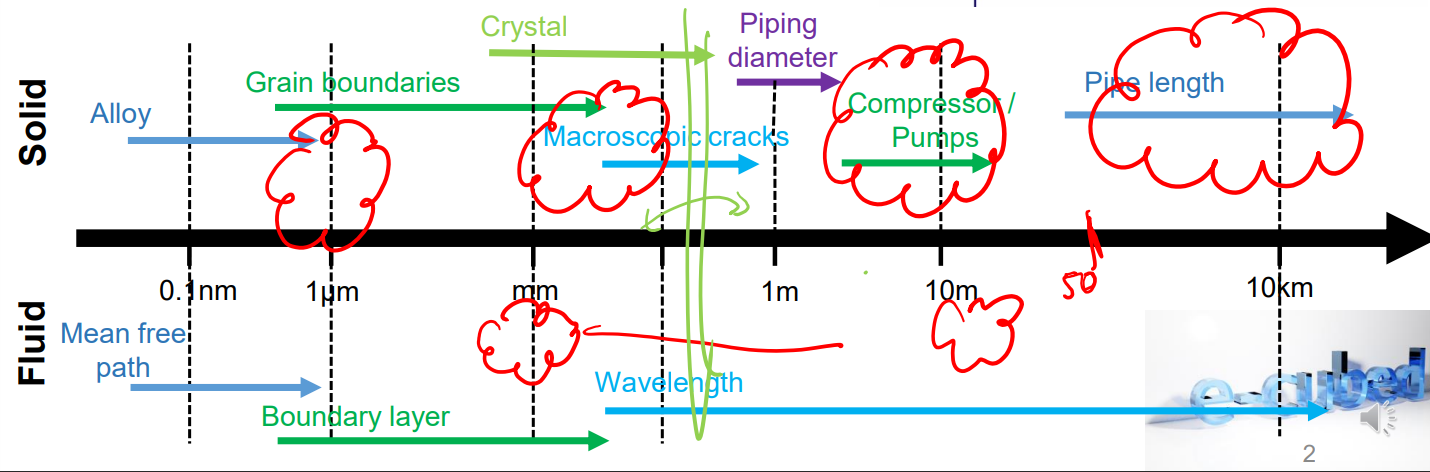
\includegraphics[width = \textwidth]{./img/figure1.png}
	\caption{Pressure pulsation in a piping system}
\end{figure}
\subsubsection{Cascade of length scales}
\begin{table}
	\begin{adjustbox}{width=\columnwidth,center}
		\begin{tabular}{@{}lll@{}}
			\toprule
			\textbf{Molecular}              & \textbf{Continuum}                            & \textbf{Structural}                     \\
			\midrule
			Material is made on this level  & Cracks operate on this level                  & Structures considered at this level     \\
			$< \SI{10}{\micro\meter}$       & $\SI{10}{\micro\meter} < x < \SI{10}{\meter}$ & $> \SI{10}{\meter}$                     \\
			Short range interactions        & Long range interactions                       & Whole scale interactions                \\
			Failure / corrosion / chemistry & Tune model - variables change                 & Long distance interaction               \\
			                                & continuously / smoothly (can account          & - vibration (waves transporting energy) \\
			                                & for discontinuous behaviour, e.g. crack)      &                                         \\
			\bottomrule
		\end{tabular}
	\end{adjustbox}
	\caption{Cascade of length scales}
\end{table}
\subsection{Complexity of the problem at different length scales}
Complexity of representation changes with the scale.
\begin{figure}[H]
	\centering
	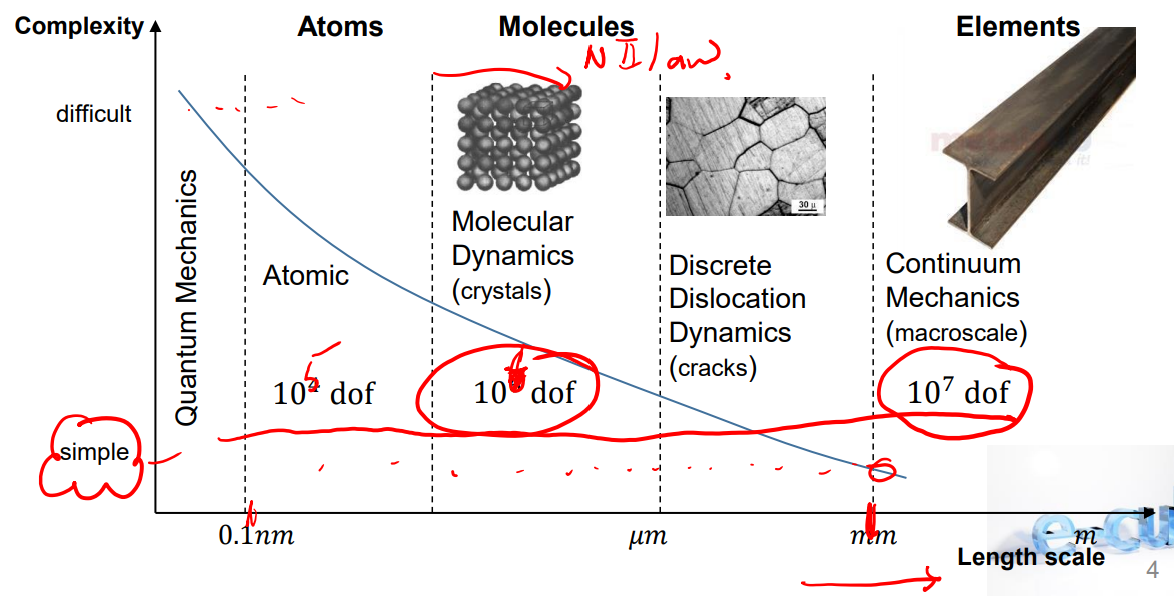
\includegraphics[width = \textwidth]{./img/figure2.png}
	\caption{Graph to show complexity against scale.}
\end{figure}
\subsection{Why focus on small scales?}
\begin{itemize}
	\item Small scale defects lead to crack initiation and propagation under external loading
	\item Failure can be corrected by changing material properties, for example, toughness
	\item Source of defects: complex chemical process (chemistry / corrosion) leads to corrosion at the surface
	\item Macroscale process is linked to microscale action
	\item Hypersonic flow - ionisation is non-continuum effect
	\item Analogy between defective liquids / solids
\end{itemize}
Note: turbulence is controlled by small vortices.
\subsubsection{Micrograph}
\begin{table}
	\centering
	\begin{tabular}{@{}ll@{}}
		\toprule
		\textbf{Domain}   & \textbf{Process}           \\
		\midrule
		Bulk              & Plasticity                 \\
		Internal boundary & Hydrogen embrittlement -   \\
		                  & plastic deformation / slip \\
		External boundary & Corrosion - chemistry      \\
		\bottomrule
	\end{tabular}
	\caption{Micrograph}
\end{table}
\begin{figure}[H]
	\centering
	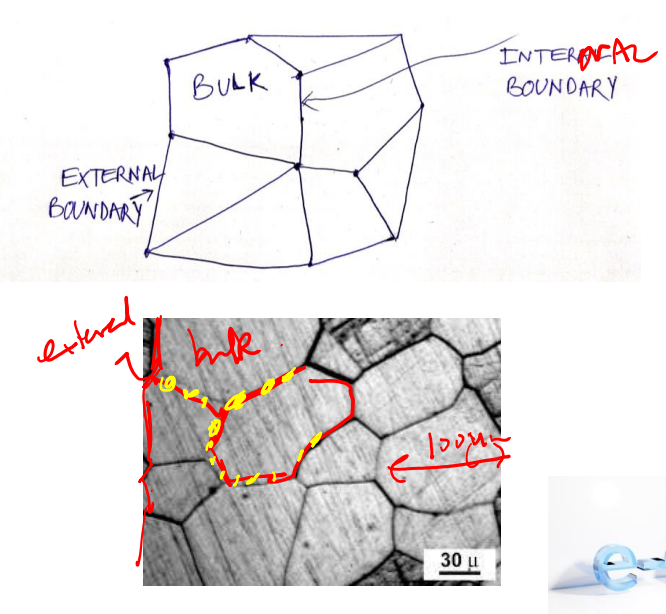
\includegraphics[width = 0.5\textwidth]{./img/figure3.png}
	\caption{Graph to show complexity against scale.}
\end{figure}
\subsubsection{Internal grain processes}
\begin{figure}[H]
	\centering
	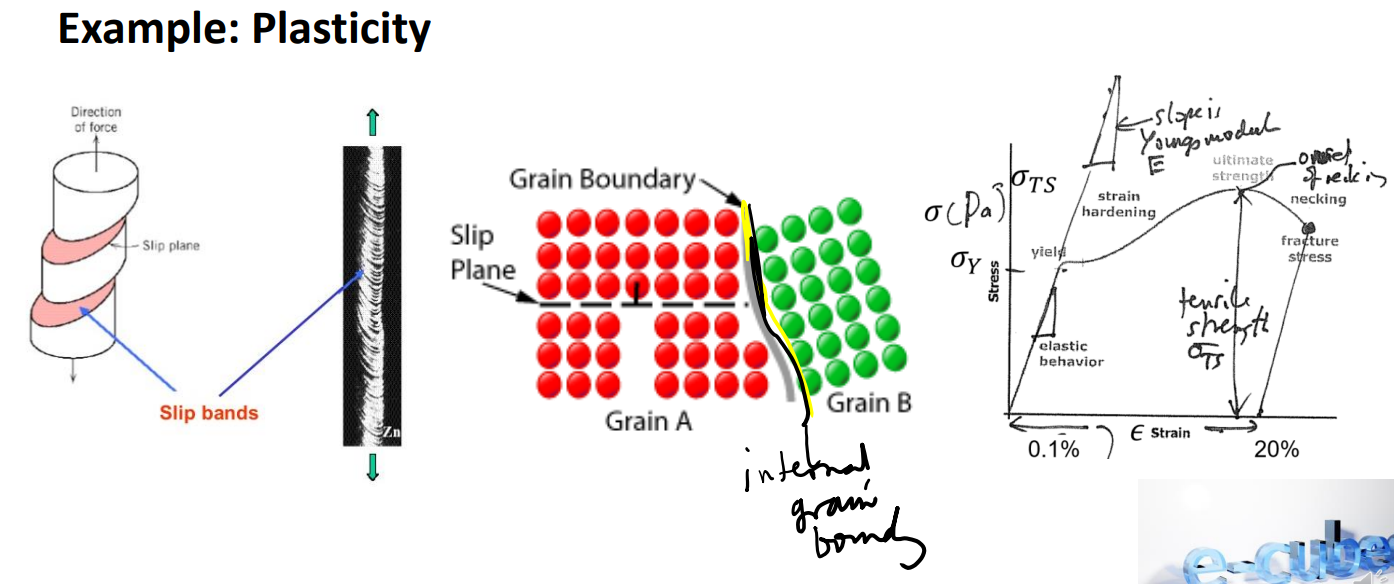
\includegraphics[width = 0.5\textwidth]{./img/figure4.png}
	\caption{Example of plasticity from internal grain process level.}
\end{figure}
\subsubsection{Internal boundary (hydrogen embrittlement - plastic deformation / slip)}
\begin{figure}[H]
	\centering
	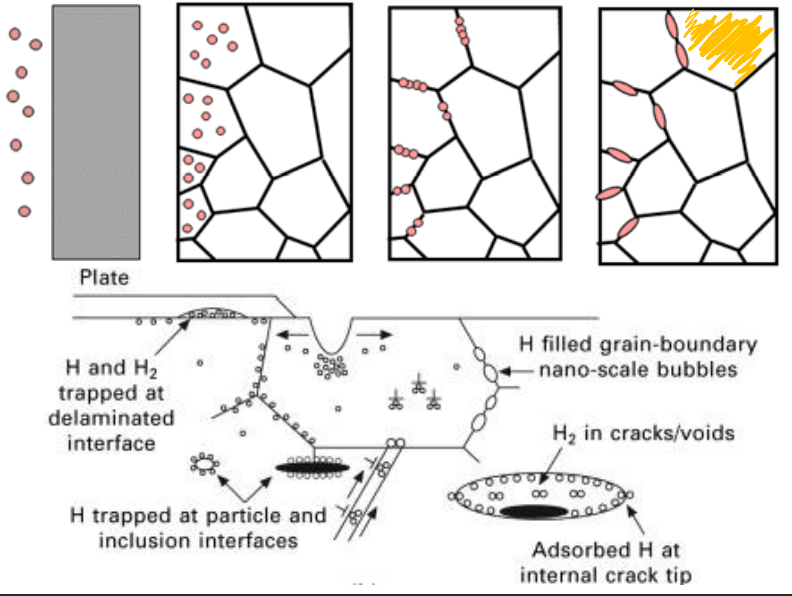
\includegraphics[width = 0.5\textwidth]{./img/figure5.png}
	\caption{Hydrogen embrittlement - plastic deformation / slip}
\end{figure}
\subsubsection{External boundary (corrosion)}
Corrosion happens over a long time and a range of scales. We need to understand how ions move around and interact with materials.
\begin{gather}
	\ce{Fe2 + (ag) + 2OH(ag) -> Fe(OH)_{2(s)}}\\
	\ce{4Fe(OH)_{2(s)} + O_{2(g)} + 2H2O_{(l)} -> Fe(OH)_{3(s)}}
\end{gather}
\begin{figure}[H]
	\centering
	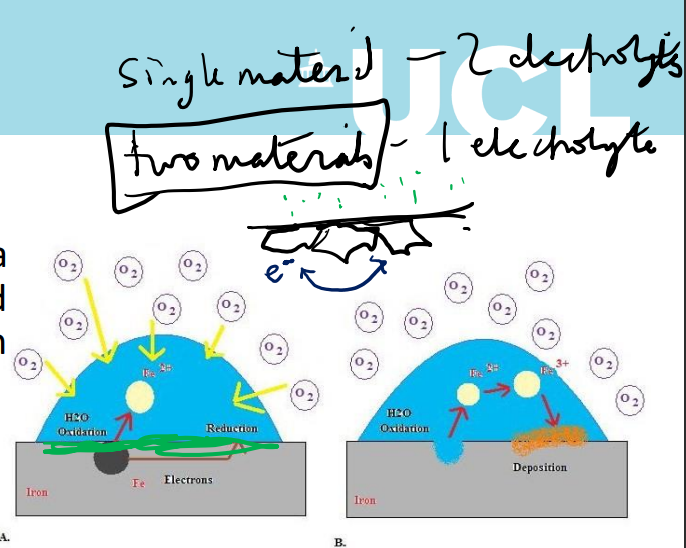
\includegraphics[width = 0.5\textwidth]{./img/figure6.png}
	\caption{Rust corrosion from grain boundary level.}
\end{figure}
\section{Categorisation of matter}
\begin{table}
	\centering
	\begin{tabular}{@{}lll@{}}
		\toprule
		\textbf{Matter} & \textbf{Modelling approach} &           \\
		\midrule
		Solid           & Atomistic                   & Continuum \\
		Gas             & Kinetic theory              & Continuum \\
		Liquid          & Molecular                   & Continuum \\
		\bottomrule
	\end{tabular}
	\caption{Categorisation of matter}
\end{table}
Switch between states are due to $p$, $V$ and $T$ and is represented by phase diagram. States of matter have been part of most religious and scientific texts for the last two thousand years, with water (aqua), fire (ignis), air (aer) and earth (terra) with the fifth being the void.
\section{Atomistic view of matter}
Typical length scale:
\begin{itemize}
	\item Diameter of atom is \SI{0.1}{\nano\meter} = \SI{1e-10}{\meter} = \SI{1}{angstrom}
	\item Nucleus diameter is \SI{1e-15}{\meter} (hydrogen) to \SI{15e-15}{\meter} (uranium-238)
\end{itemize}
\subsection{Bulk characteristic of materials}
The aim is to understand the relationship between the macrostructure and the microstructure. Key measures are:
\begin{itemize}
	\item Young's modulus $E = \left. \frac{\dif \sigma}{\dif \varepsilon} \right|_{\varepsilon \rightarrow 0}$
	\item Tensile stress: $\sigma_{TS}$
	\item Yields stress: $\sigma_{Y}$
	\item Ductility: $\epsilon_{T}$
\end{itemize}
It is important to understand the following:
\begin{table}
	\centering
	\begin{tabular}{@{}lll@{}}
		\toprule
		\textbf{Properties} &                                   & \textbf{Definition}                                \\
		\midrule
		Elastic modulus     & $E$ (\si{\pascal})                & Measure of material resistance to deformation.     \\
		Yield stress        & $\sigma_Y$ (\si{\pascal})         & Measure of stress at which the elastic behaviour   \\
		                    &                                   & disappears and plastic behaviour initiates.        \\
		Hardness            & HBW                               & Measure of material resistance to indentation      \\
		Creep               &                                   & Time-dependant deformation at high temperature     \\
		                    &                                   & and constant stress.                               \\
		Toughness           & $K$ (\si{\joule\per\meter\cubed}) & Resistance to crack propagation.                   \\
		Ductility           & $\epsilon_T$                      & Material's ability to undergo plastic deformation. \\
		\bottomrule
	\end{tabular}
	\caption{Key points on material properties}
\end{table}
How are they related to the microstructure?
\subsection{Newtonian model of matter}
Useful for biological, physical problems, solids, liquids and gases. This is based on a description of matter as a collection of point particles, an approach that is useful for gases, liquid and solids. The dynamics of the i-th molecule is:
\begin{gather}
	\underline{F}_i = \sum_{j,j} \neq \nabla U\left(x_i,x_j\right)
\end{gather}
Located at point $\underline{x}_i$ whose dynamics are:
\begin{gather}
	m_i \dfrac{\dif \underline{v}_i}{\dif t} = \underline{F}_i\\
	\underline{v}_i = \frac{\dif \underline{x}_i}{\dif t}
\end{gather}
The formulation requires the form of the interaction stated using the Lennard-Jones 6-12 potential:
\begin{gather}
	U = 4 \epsilon \left(\left(\frac{\sigma}{r}\right)^{12} - \left(\frac{\sigma}{r}\right)^6\right) + \dots
\end{gather}
The difficultly is that neighbourhood lists are kept and only sum over local interaction of molecules.
\begin{itemize}
	\item Not hard collision
	\item Time stepping fixed
	\item Potentials can be empirical or chosen to now slow down calculations
\end{itemize}
\begin{gather}
	U = U_{stretch} + U_{bend} + U_{torsion} + U_{vanderWaal} + U_{electro} + U_{cross}
\end{gather}
Research gaps:
\begin{itemize}
	\item Link between continuum and molecular
	\item Quantum - mechanical models
\end{itemize}
\subsection{Vibrational modes and energy}
Mechanical representation of matter. Molecules interact with their neighbours and fields. Interaction may be quite far, particularly when charges are important. We are familiar with how degrees of freedom influence properties of a gas, especially through the isentropic index. Energy is stored in various modes of vibration e.g. gas. This is called classical molecular dynamics.
\subsection{Molecular description of material properties}
\subsubsection{Primary bonds}
Ionic and covalent bonds are extremes with most (electron distribution) bonds lying between (polar covalent)
\begin{figure}[H]
	\centering
	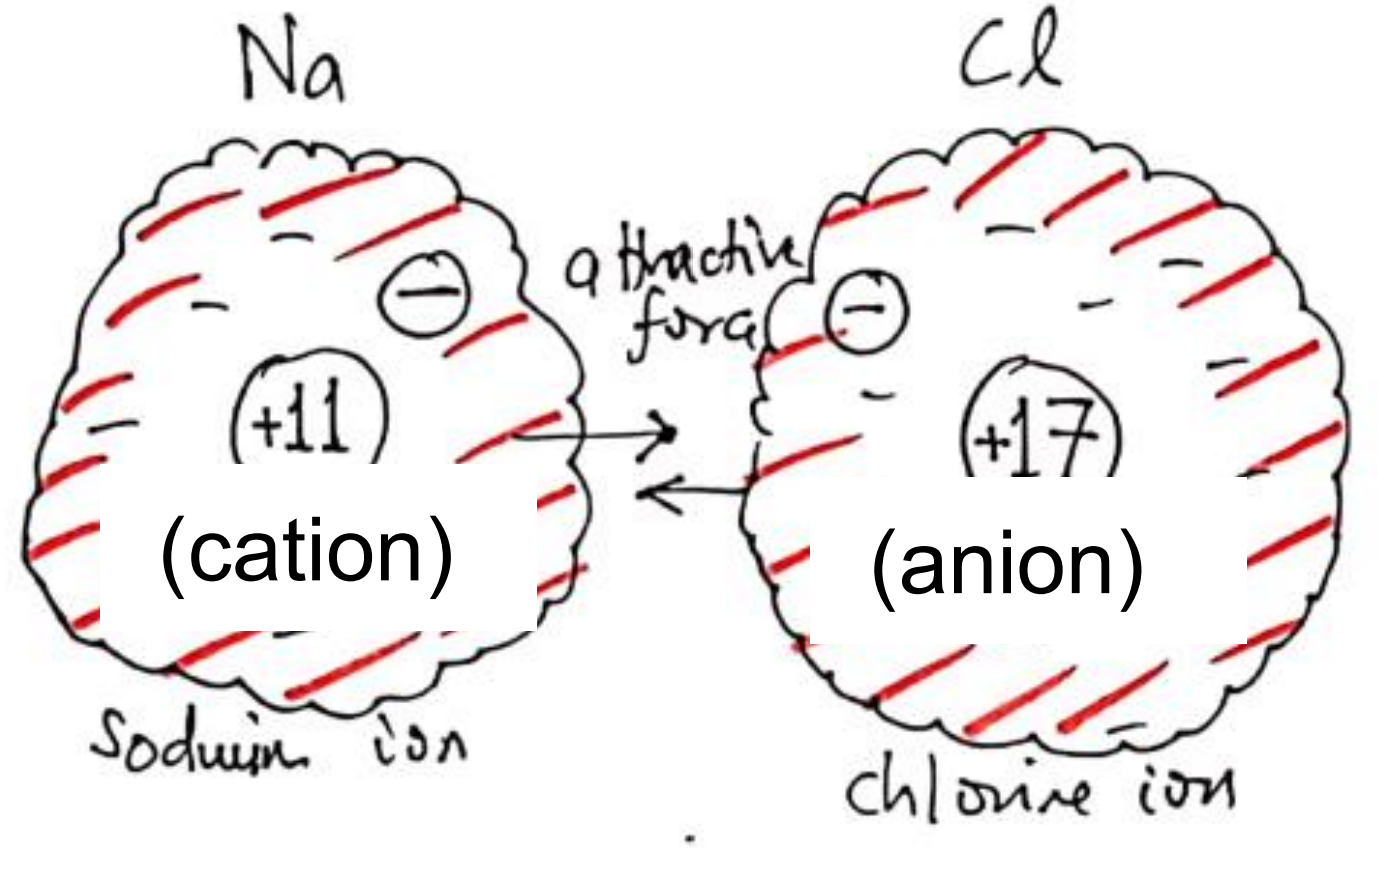
\includegraphics[width = 0.5\textwidth]{./img/figure7.png}
	\caption{Ionic bond (electrovalence)}
\end{figure}
\begin{gather}
	F = \frac{q_1 q_2}{4\pi \epsilon_0 r^2}\\
	U = U_i - \frac{q^2}{4\pi\epsilon_0 r} + \frac{B}{r^n}
\end{gather}
\begin{figure}[H]
	\centering
	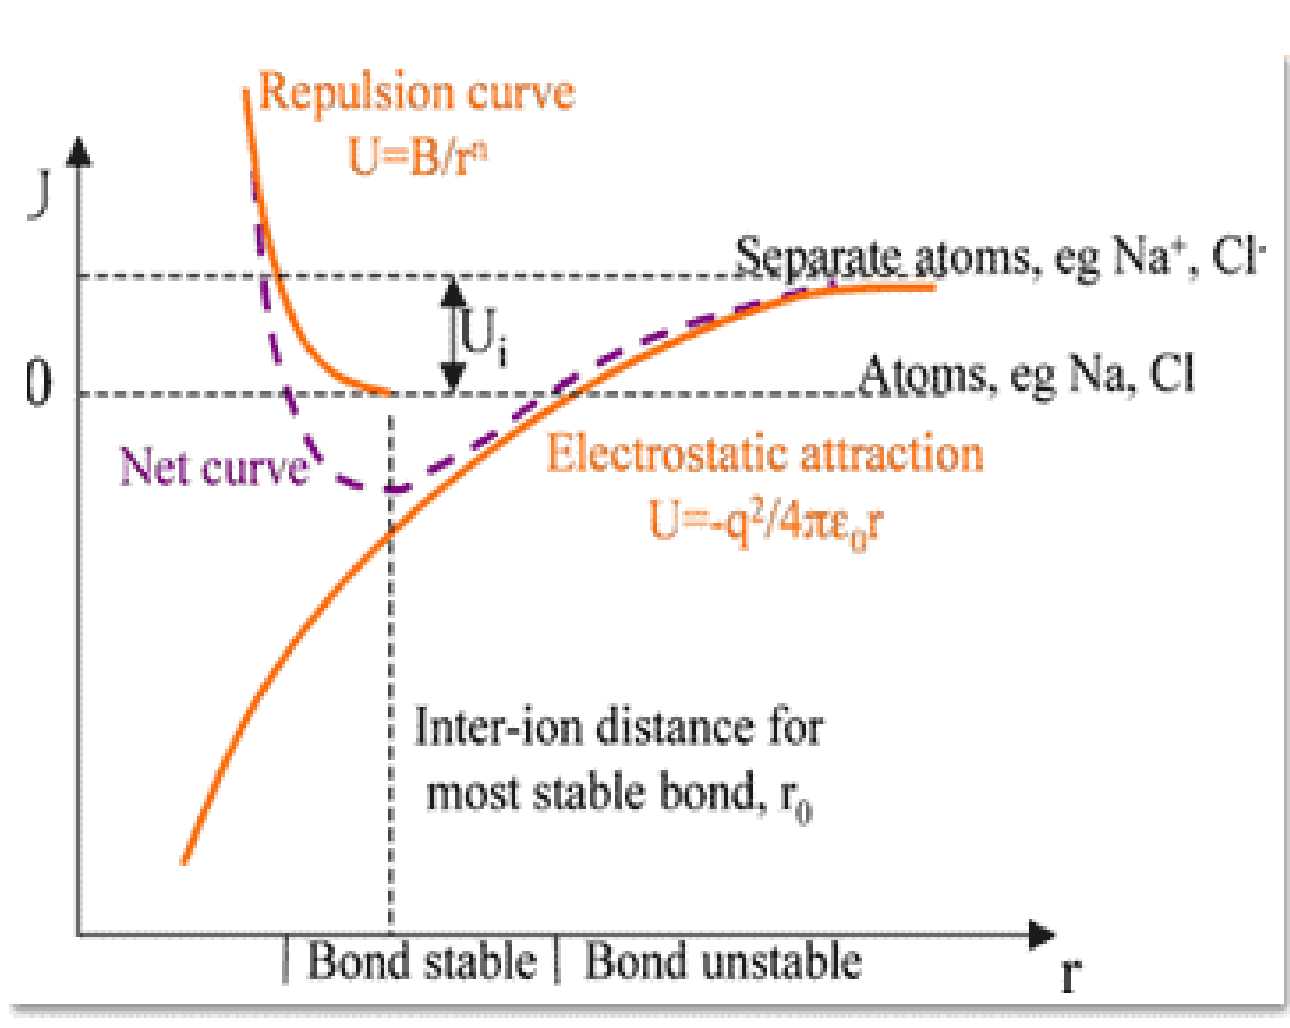
\includegraphics[width = 0.5\textwidth]{./img/figure8.png}
	\caption{Bond stability.}
\end{figure}
\begin{figure}[H]
	\centering
	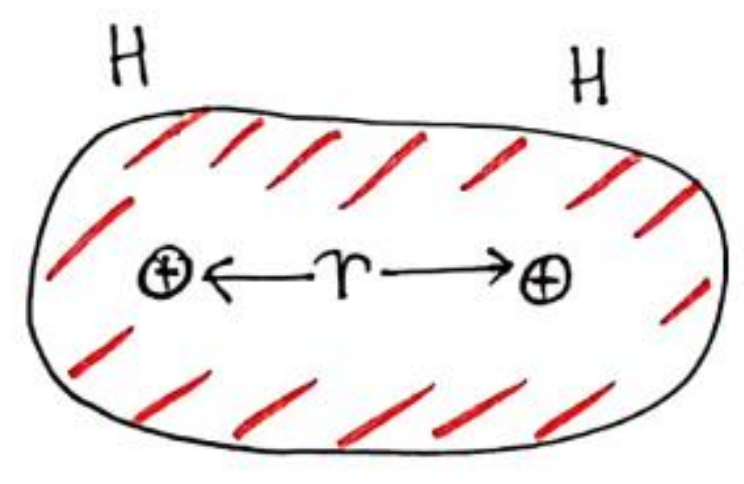
\includegraphics[width = 0.5\textwidth]{./img/figure9.png}
	\caption{Covalent bond (covalence). Note the overlap of electron orbit.}
\end{figure}
\begin{gather}
	U = -\frac{A}{r^m} + \frac{B}{r^n}, \, m<n
\end{gather}
\begin{figure}[H]
	\centering
	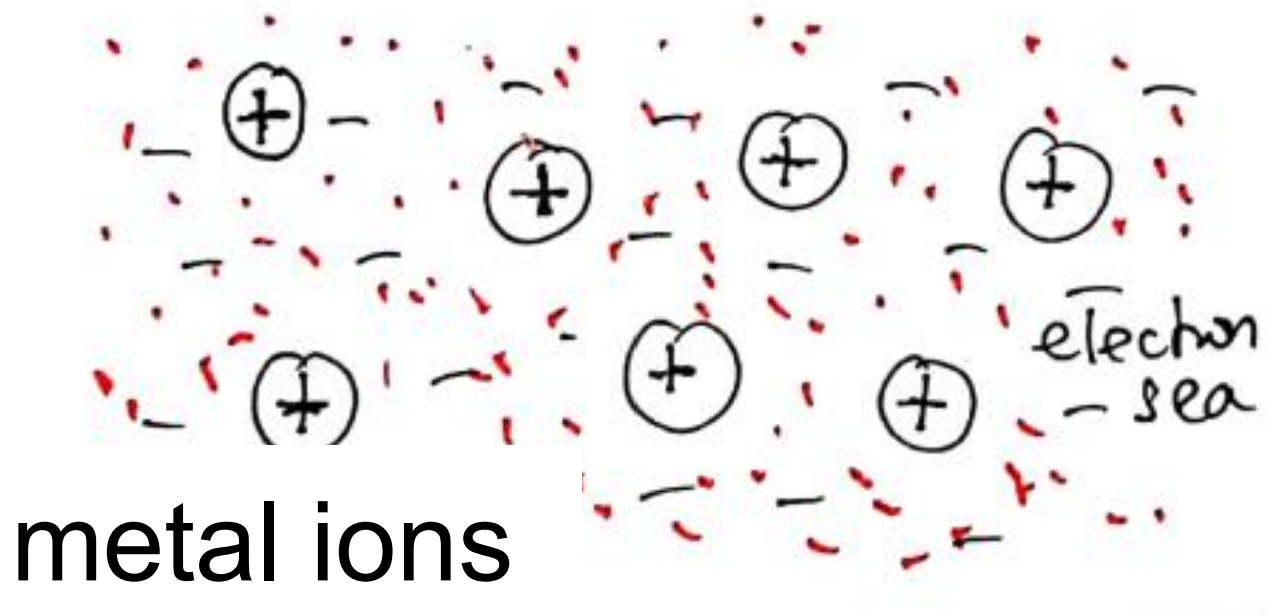
\includegraphics[width = 0.5\textwidth]{./img/figure10.png}
	\caption{Metallic bond (electron cloud).}
\end{figure}
\begin{gather}
	e = \SI{1.6e-19}{C}\\
	\epsilon_0 = \SI{8.8e-12}{Nm^2C^{-2}}\\
	\SI{1}{eV} = \SI{1.6e-19}{J}
\end{gather}
\subsubsection{Secondary bonds}
The secondary bonds are important - without them many gases would not condense. The relative displacement of the positive and negative charge gives rise to a dipolar force. This gives rise to an attractive force. Most usual form is the Lennard Jones 6-12 potential.
\begin{gather}
	U = -\frac{A}{r^6} + \frac{B}{r^n}
\end{gather}
\begin{figure}[H]
	\centering
	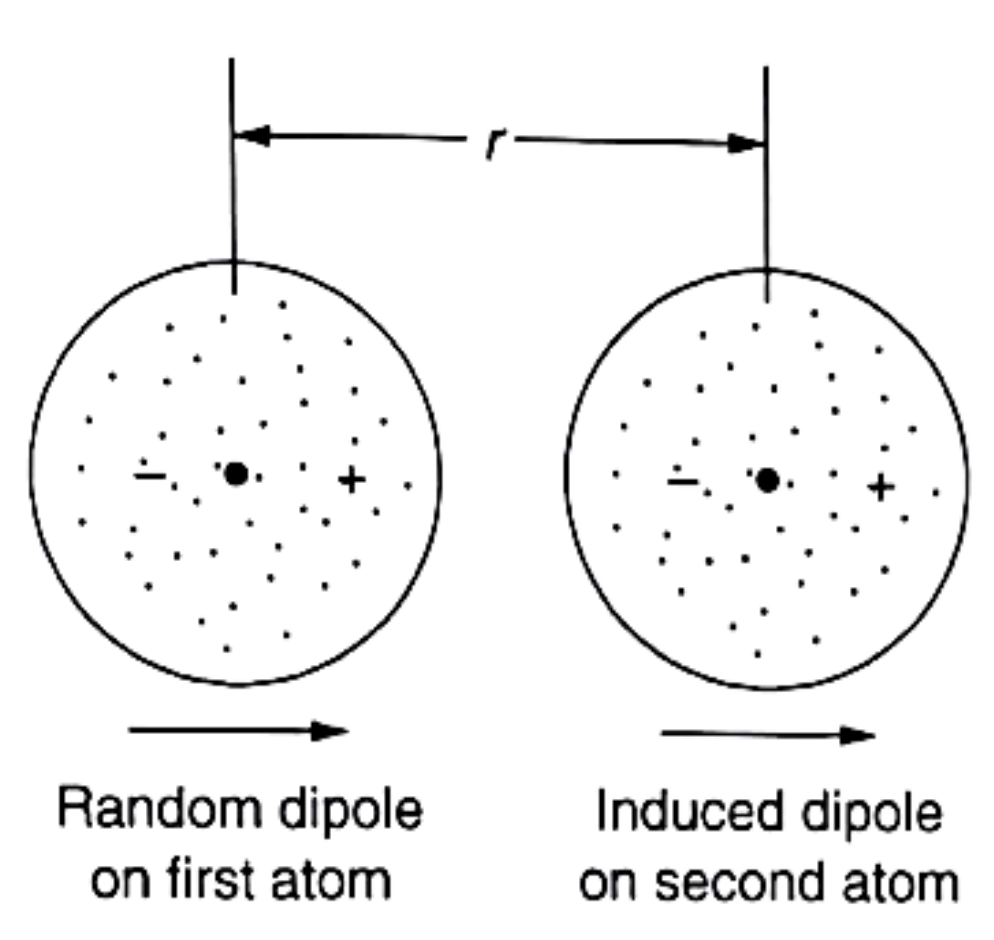
\includegraphics[width = 0.5\textwidth]{./img/figure11.png}
	\caption{Secondary bonds. Note: long range attractive force -  dipole-dipole interactions. Overlapping electron orbits - repulsive.}
\end{figure}
\subsubsection{Physical basis of Young's Modulus}
Classical mechanics:
\begin{gather}
	m\frac{\dif v}{\dif t} = \frac{\dif U }{\dif r}
\end{gather}
where $U$ is the potential energy. At equilibrium:
\begin{gather}
	\frac{\dif U}{\dif r } = 0
\end{gather}
so that close to this point, the energy potential can be expanded to give:
\begin{gather}
	m \frac{\dif^2 r }{\dif t^2} = \left(\frac{\dif^2 U}{\dif r^2}\right)\left(r-r_0\right)
\end{gather}
Around equilibrium point:
\begin{gather}
	F = S_0 \left(r - r_0\right)\\
	S_0 = -\frac{\dif^2 U}{\dif r^2}
\end{gather}
The stress is:
\begin{gather}
	\sigma = N S_0 \left(r - r_0\right) = \frac{S_0\left(r-r_0\right)}{r_0^2}
\end{gather}
The Young's modulus is:
\begin{gather}
	E = \frac{\sigma}{\epsilon} = \frac{S_0}{r_0}
\end{gather}
Estimate:
\begin{gather}
	S_0 = \frac{\alpha q^2}{4\pi\epsilon_0r^2}\\
	E = \frac{\sigma}{\epsilon} = - \frac{\frac{\dif^2 U}{\dif r^2}}{r_0} = \frac{\delta e^2}{4\pi\epsilon_0r_0^4}
\end{gather}
Atom spacing:
\begin{gather}
	\overline{r}_0 \approx 8.54
\end{gather}
\begin{figure}[H]
	\centering
	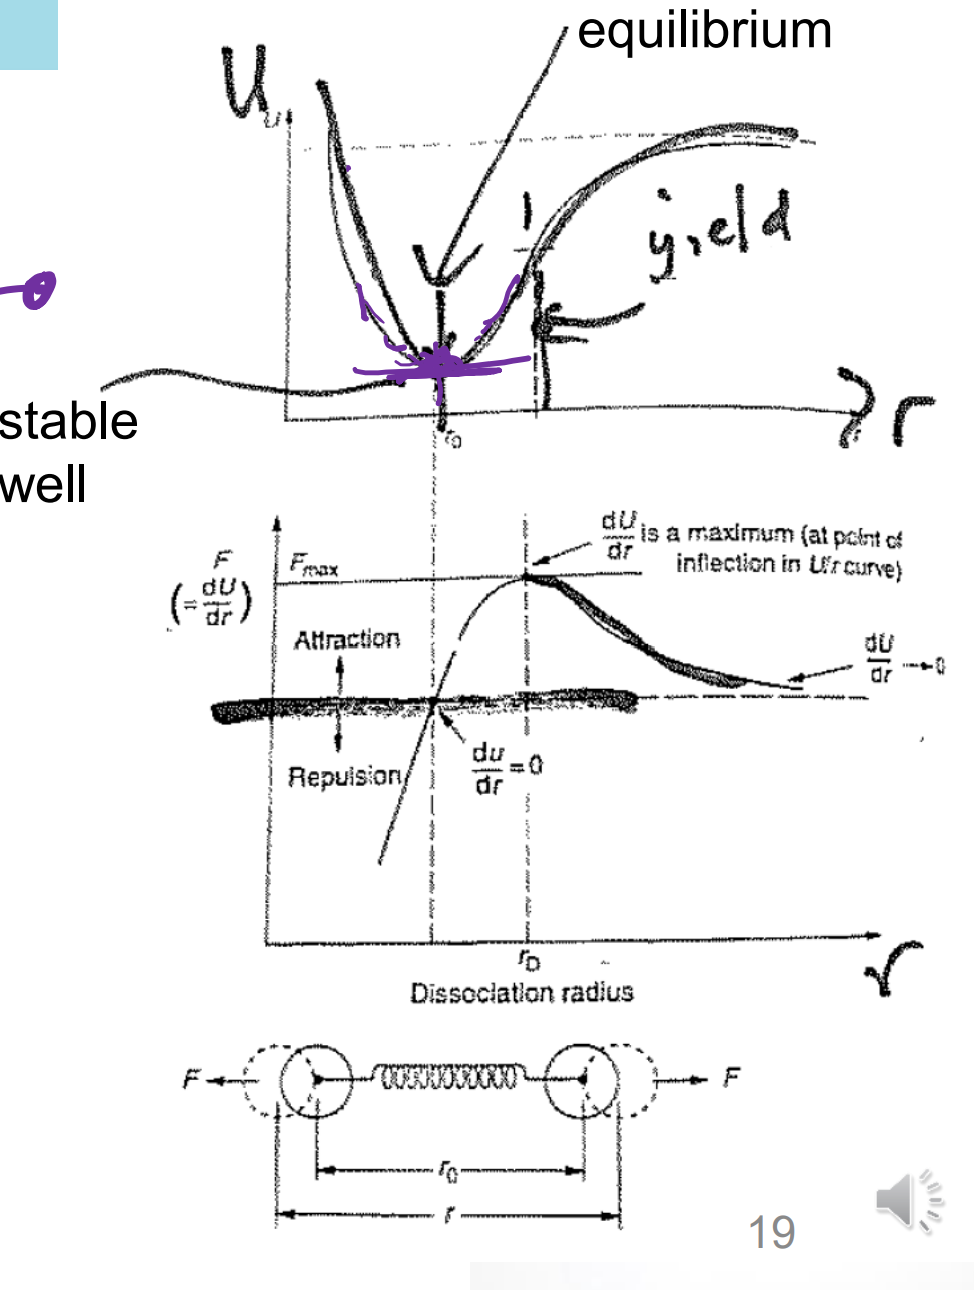
\includegraphics[width = 0.5\textwidth]{./img/figure12.png}
	\caption{Young's modulus from atomic perspective.}
\end{figure}
\subsubsection{Comparison between molecular and macroscopic measurements}
\begin{table}[H]
	\centering
	\begin{tabular}{@{}llll@{}}
		\toprule
		\textbf{Bond type} & $S_0$ / \si{Nm^{-1}} & \textbf{Young's modulus estimate} & \textbf{Measurement}       \\
		                   &                      & $E$ / \si{\giga\pascal}           &                            \\
		\midrule
		Covalent           & 50 - 180             & 200 - 1000                        & 1000 (diamond)             \\
		Metallic           & 15 - 75              & 60 - 300                          & 200 (nickel)               \\
		Ionic              & 8 - 24               & 32 - 96                           & 15 - 91 (alkali halides)   \\
		H-Bond             & 2 - 3                & 8 - 12                            & 9.1 (ice)                  \\
		van der Waals      & 0.5 - 1              & 2 - 4                             & 0.01 - 2 (rubber to nylon)
	\end{tabular}
	\caption{Comparison between molecular and macroscopic measurements.}
\end{table}
\subsubsection{Estimation of yield stress}
Returning to the molecular model since:
\begin{gather}
	U = \epsilon \left(-\frac{A}{r^6} + \frac{B}{r^{12}}\right)\\
	U'' = \epsilon \left(- \frac{6\times 7A}{r^8} + \frac{12\times 13B}{r^{14}}\right)
\end{gather}
Then, maximum stress is:
\begin{gather}
	\sigma_Y \approx \frac{E}{8}
\end{gather}
Therefore:
\begin{gather}
	\frac{\sigma_Y}{E} ~ \frac{1}{8}
\end{gather}
This estimated ratio is good for ceramics, but not good for metals. So what is missing from a molecular description?
\begin{figure}[H]
	\centering
	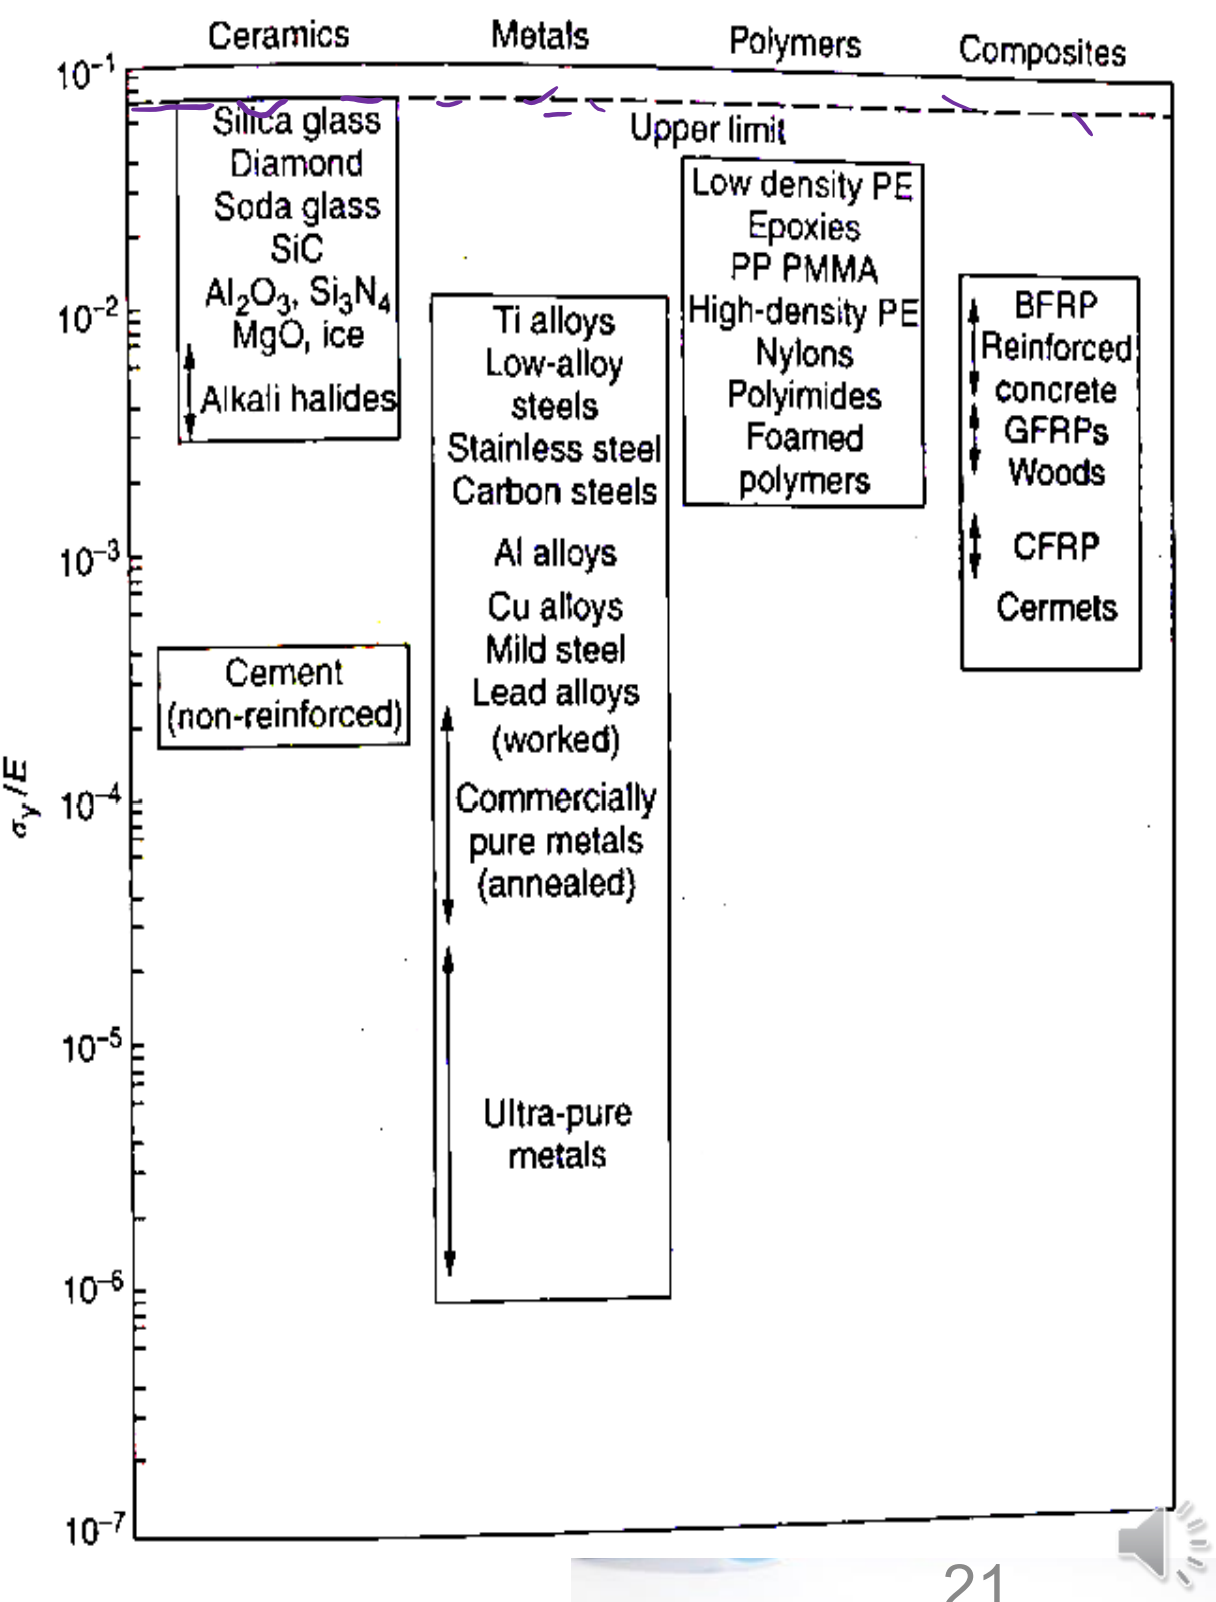
\includegraphics[width = 0.5\textwidth]{./img/figure13.png}
	\caption{Graph to show yield stress ratio for different materials.}
\end{figure}
\subsection{Material classification}
\begin{itemize}
	\item Metals
	      \begin{itemize}
		      \item Ferrous metals and alloys
		      \item Non ferrous metals and alloys
		      \item (focus on here)
	      \end{itemize}
	\item Polymeric (non metallic, non crystalline)
	      \begin{itemize}
		      \item Thermoplastic plastics
		      \item Thermoset plastics
		      \item Elastomers
	      \end{itemize}
	\item Ceramics
	      \begin{itemize}
		      \item Glass
		      \item Diamond
		      \item Glass ceramics
	      \end{itemize}
	\item Composites (everything else)
	      \begin{itemize}
		      \item Metal-matrix composites
		      \item Sandwich structures
		      \item Concrete
	      \end{itemize}
\end{itemize}
\subsubsection{Three common configurations}
\begin{table}[H]
	\centering
	\begin{tabular}{@{}llll@{}}
		\toprule
		\textbf{Type} & \textbf{Name}               & \textbf{Description}      & \textbf{Example}             \\
		\midrule
		BCC           & Body centred cube - 2 atoms & Harder and less malleable & Lithium, Sodium, Potassium   \\
		              &                             & Packing factor 0.68       & Chromium, Barium, Alpha-iron \\
		FCC           & Face centred cube           & malleable, softer 0.74    & Copper, Gold, Aluminium      \\
		              &                             &                           & Iridium, Lead, Nickel, etc.  \\
		HCP           & Hexagonal close packed      & 6 atoms                   & Cadmium, Magnesium, Titanium \\
		              &                             & Packing ratio 0.74        & Zinc, Zirconium              \\
		\bottomrule
	\end{tabular}
	\caption{Configurations of atoms.}
\end{table}
\subsubsection{Solidification and crystal growth}
Under normal circumstances, crystal growth starts at many nucleation points. Solidification leads to crystals growing and stop growing when they meet another crystal. A crystal is usually called a grain. The boundary between grains is the grain boundary where structure is disordered. This is controlled using nucleation points and directional solidification and liquid freezing-dendritic growth and shrinkage occurs during cooling.
\begin{figure}[H]
	\centering
	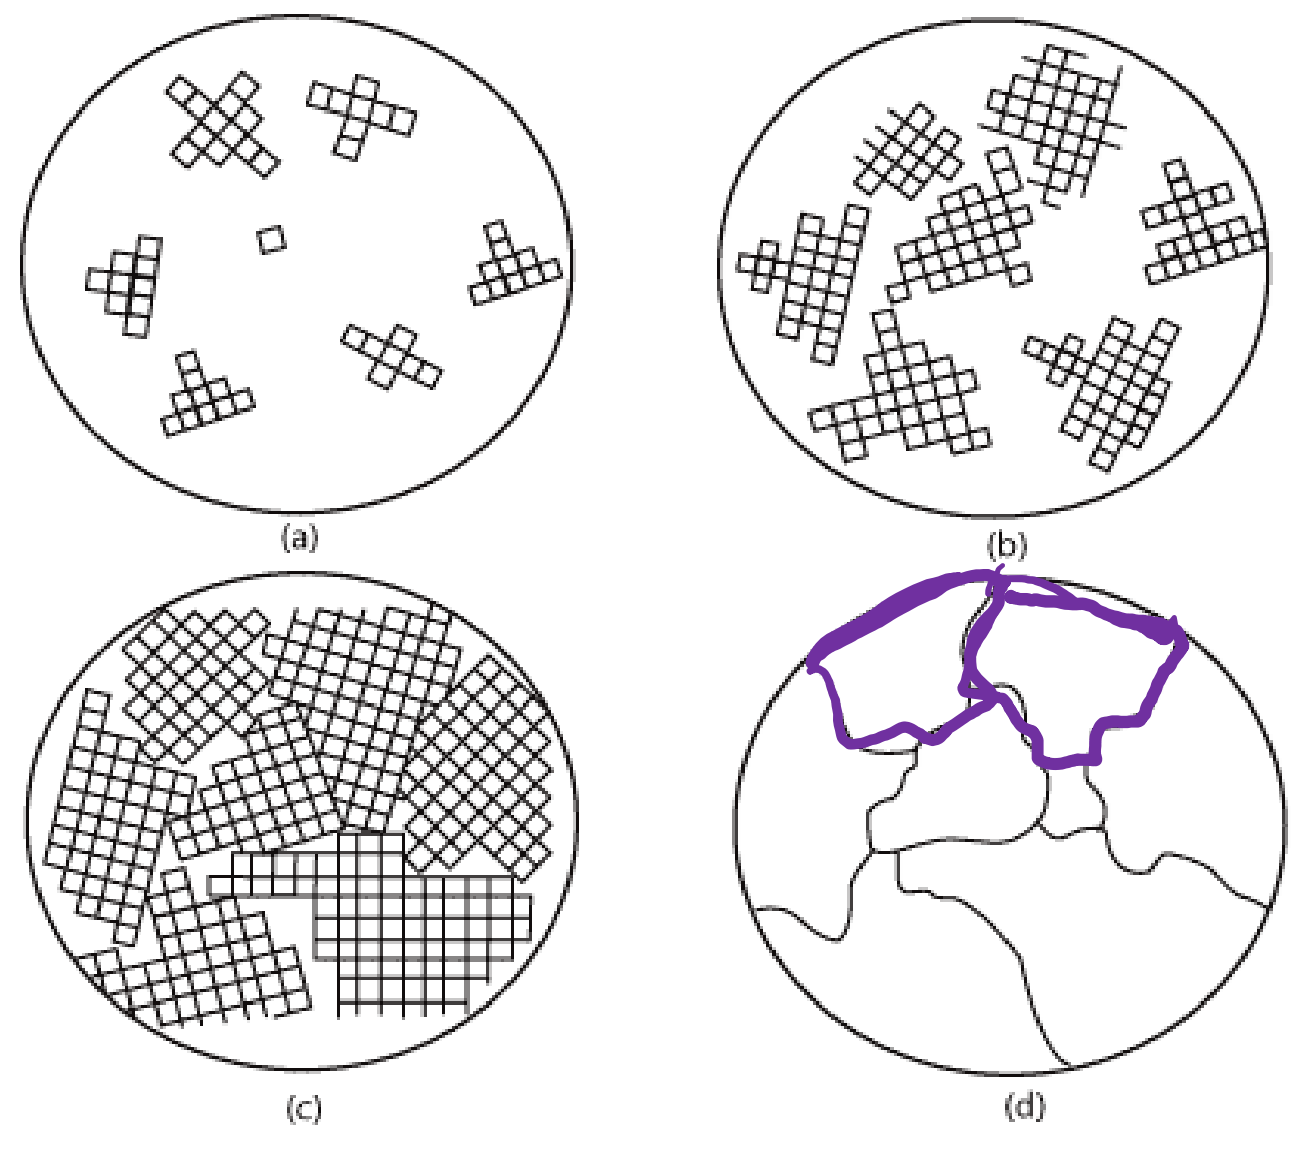
\includegraphics[width = 0.6\textwidth]{./img/figure14.png}
	\caption{Nucleation of crystals.}
\end{figure}
\subsubsection{Crystal defects}
Three types of defects:
\begin{enumerate}
	\item Point defects: which are places where an atom is missing or irregularly placed in the lattice structure. Point defects include lattice vacancies, self interstitial atoms, substitution impurity atoms and interstitial impurity atoms
	\item Linear defects: which are groups of atoms in irregular positions. Linear defects are commonly called dislocations
	\item Planar defects: which are interfaces between homogeneous regions of the material. Planar defects include grain boundaries, stacking faults and external surfaces
\end{enumerate}
\subsubsection{Atomistic view of plastic deformation}
Elastic deformation - stress is small, the metal can recover to initial state when the stress is removed. This involves stretching the bonds but atoms do not mover over one another.

Plastic deformation - stress is large, plastic deformation involves the breaking of a limited number of atomic bonds by the movement of dislocations. Since the energy required to move is lowest along the densest planes of atoms, dislocations have a preferred direction of travel within a grain of the material. This results in slip that occurs along parallel planes within the grain. These parallel slip planes group together to form slip bands. A slip band appears as a single line under the microscope, but it is in fact made up of closely spaced parallel slip planes as shown in the image.
\begin{figure}[H]
	\centering
	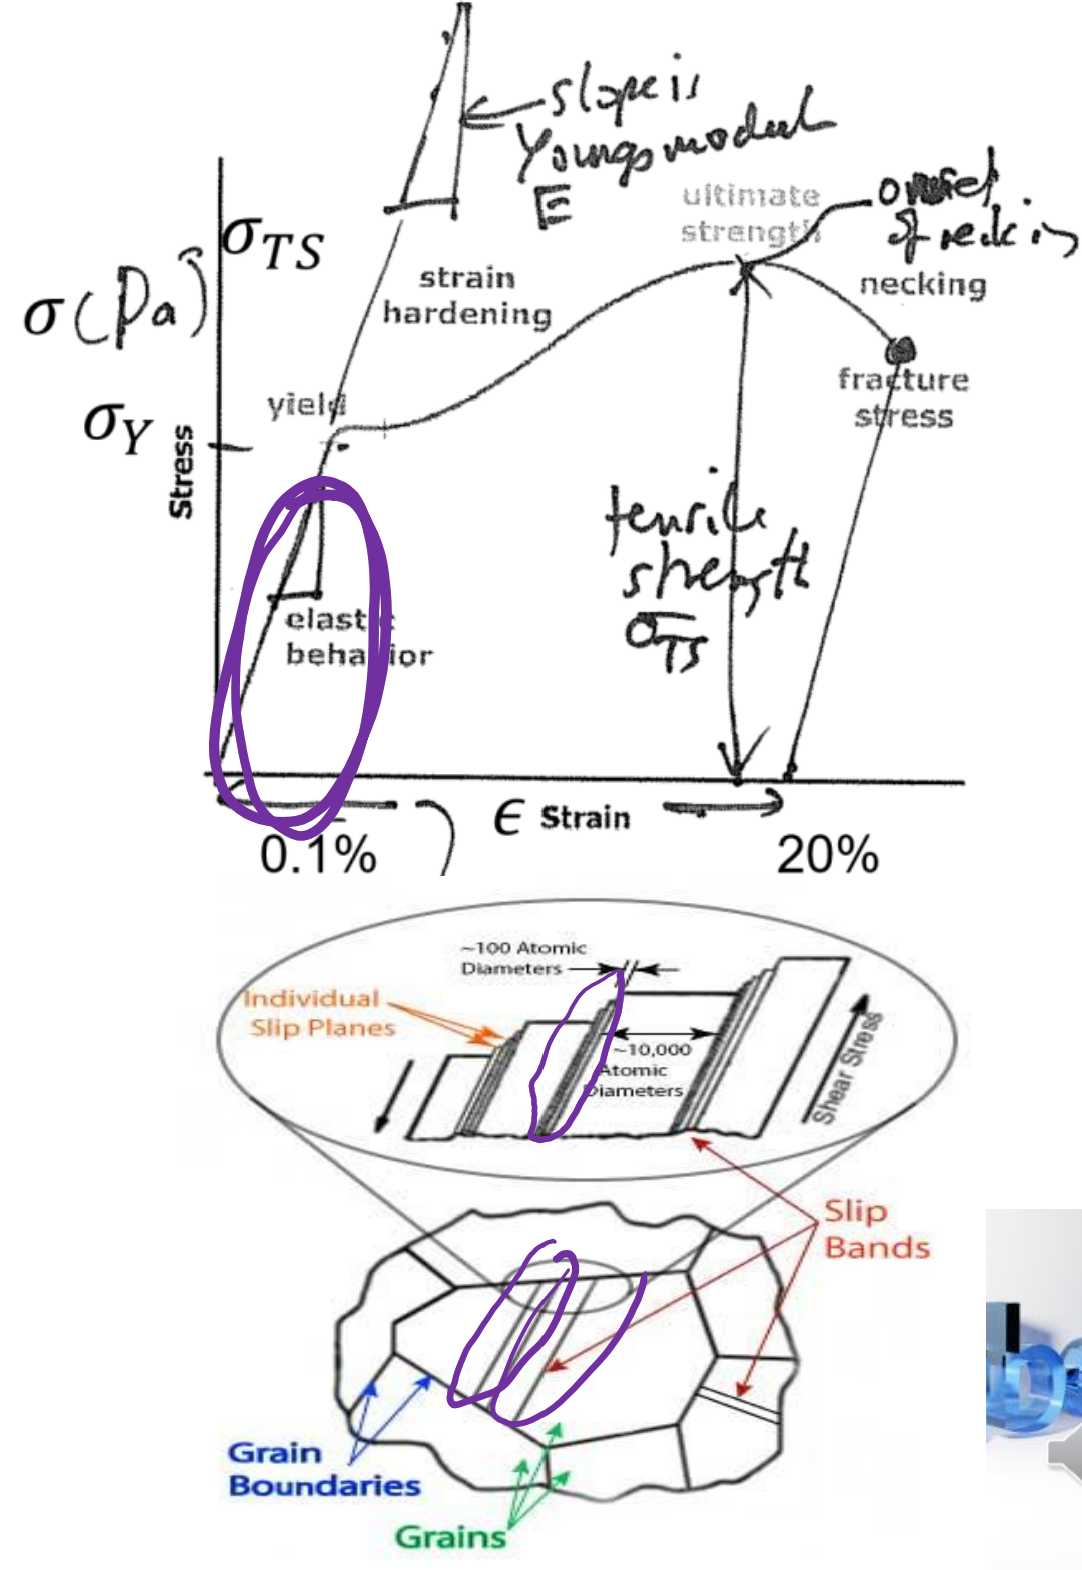
\includegraphics[width = 0.5\textwidth]{./img/figure15.png}
	\caption{Stress-strain curve.}
\end{figure}
\subsubsection{Fatigue crack initiation}
The life of a fatigue crack has two parts, initiation and propagation. Dislocations play a major role in the fatigue crack initiation phase. It has been observed in laboratory testing that after a large number of loading cycles dislocation pule up and form structures called persistent slip bands. Initiation has a molecular origin.
\subsubsection{Topological change in crystal structure}
\begin{figure}[H]
	\centering
	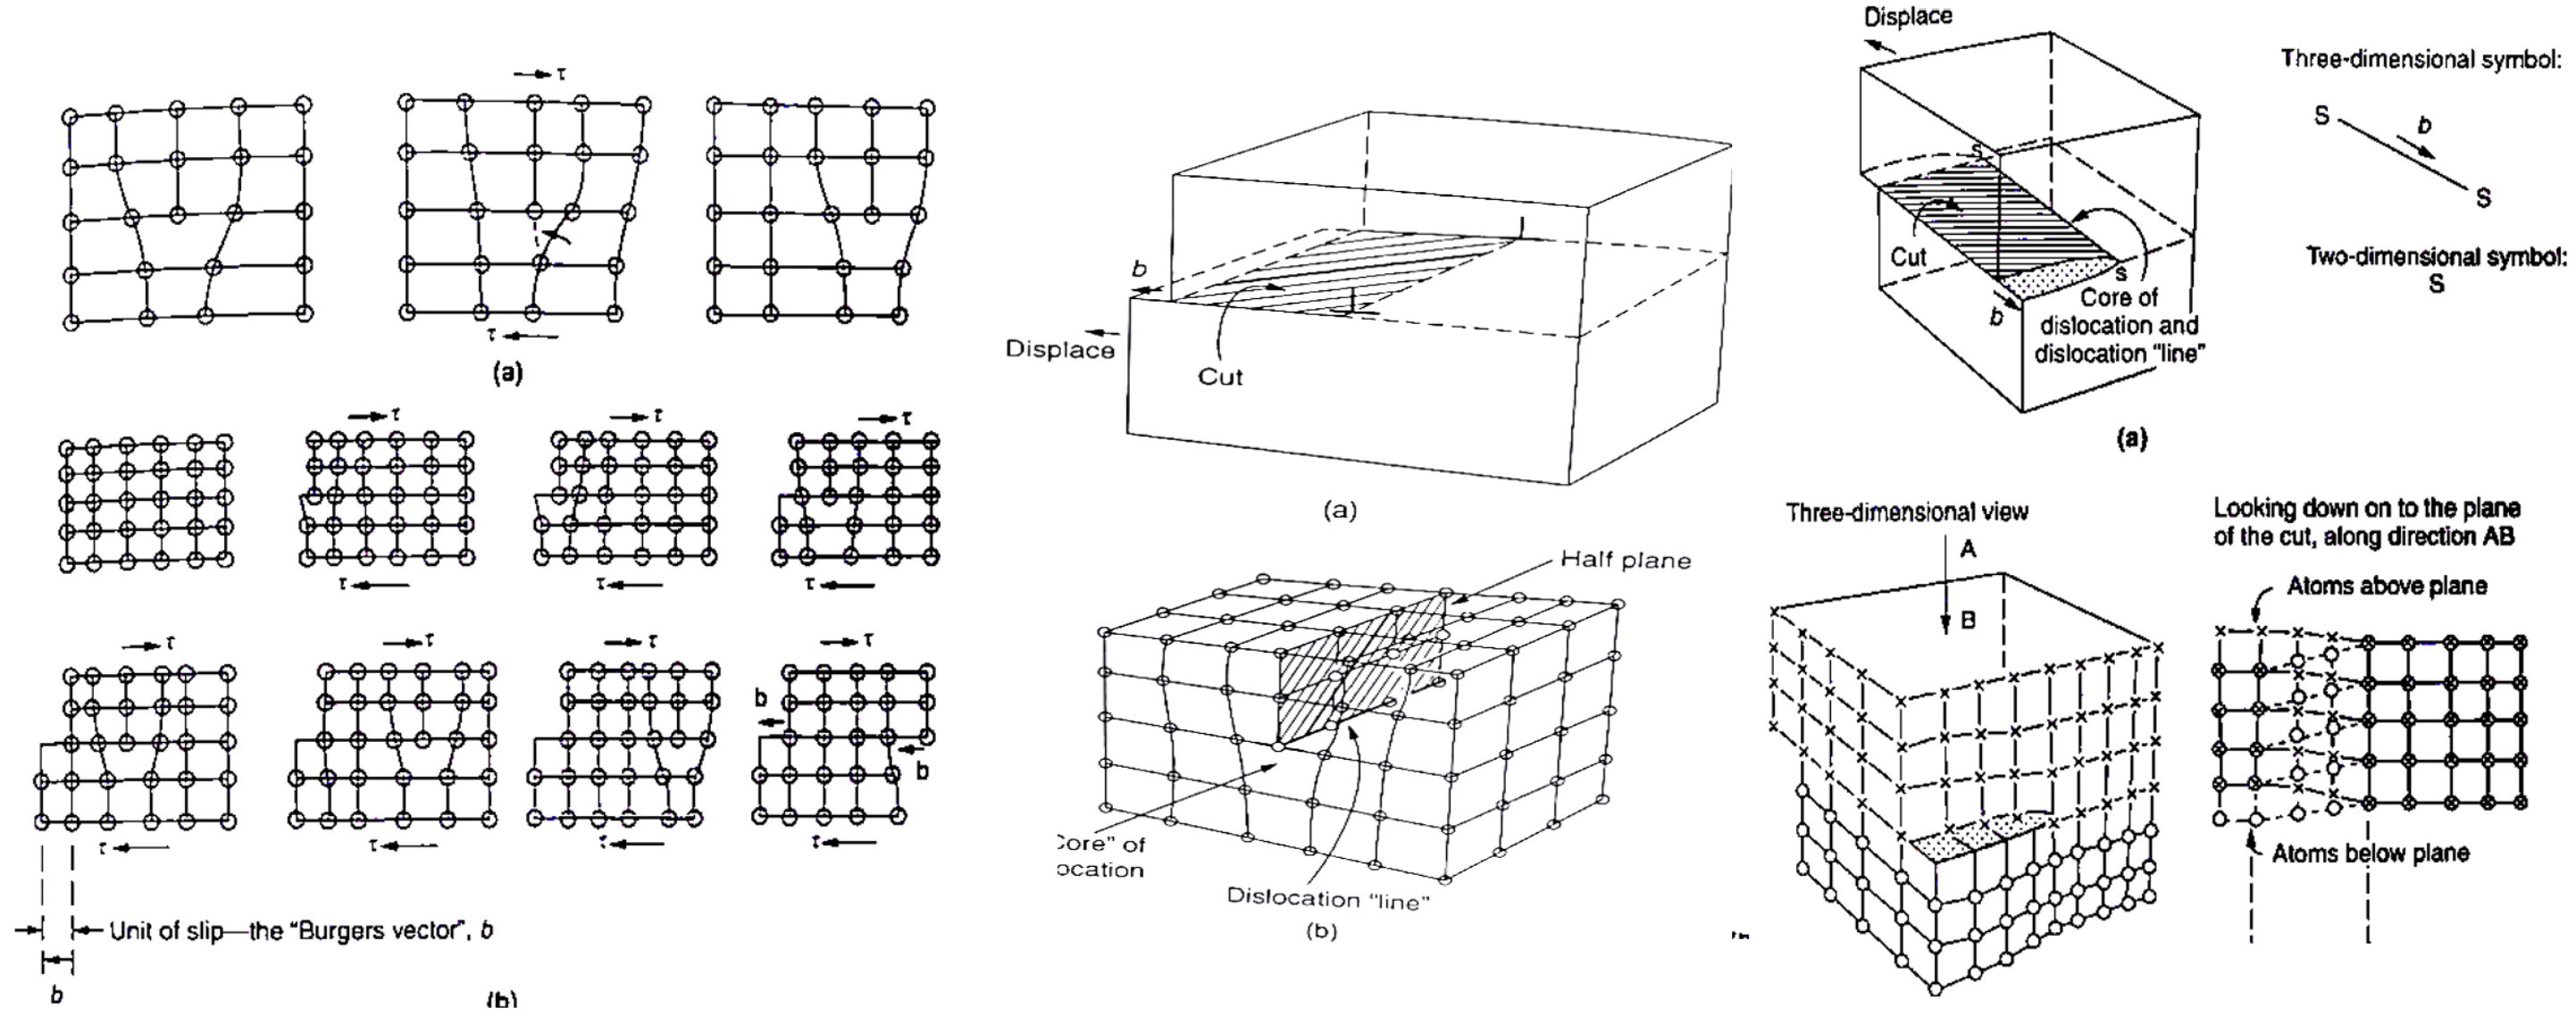
\includegraphics[width = 0.5\textwidth]{./img/figure16.png}
	\caption{Topological changes in crystal structure.}
\end{figure}
\section{Kinetic theory of gases}
Statistical 19th century view of macroscopic properties of gas. Boltzmann and colleagues developed new techniques to describe matter. Heavily influenced the theory of turbulence $\leftarrow$ based on kinetic theory of a gas.

$p = \rho RT$ origin with statistical theory.

This is an excellent macroscopic model of matter. The problem is that it does not work well for low pressure, high pressure or when density is low (and continuum concepts don't work).
\subsection{Speed of molecules}
Results tell us about average speed but not the distribution.
\begin{gather}
	n_v\left(E\right) = n_0 e^{-\frac{E}{k_B T}}
\end{gather}
where, $n_v\left(E\right)$ is the Boltzmann distribution which coups a lot. The speed of the molecules satisfies the Maxwell-Boltzmann distribution.
\begin{gather}
	f\left(v\right) = 4\pi \left(\frac{m}{2\pi k_B T}\right)^3 v^2 \exp{\left(-\frac{mv^2}{2k_B T}\right)}
\end{gather}
\begin{figure}[H]
	\centering
	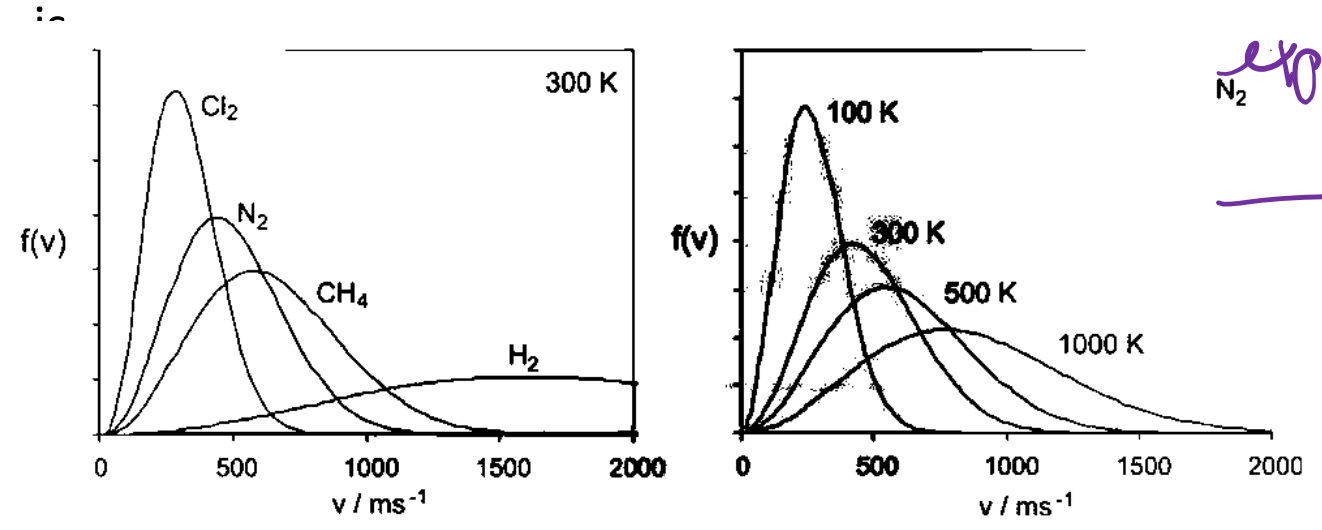
\includegraphics[width = 0.7\textwidth]{./img/figure17.png}
	\caption{Speed of molecules.}
\end{figure}
\subsection{Equations of state of real gases}
The molecular continuum view of matter are linked. Virial equation:
\begin{gather}
	pV = nRT\left(1 + \frac{B}{V_m} + \frac{C}{V_m^2} + \dots\right)
\end{gather}
where $B$, $C$ are the second and third virial coefficients. Van der Waals equation:
\begin{gather}
	\left(p + a\frac{n^2}{V^2}\right)\left(V - nb\right) = nRT \textrm{ or}\\
	P = \frac{nRT}{V- nb} - a \frac{n^2}{V^2}
\end{gather}
$n$ is the number of moles. $nb$ is the volume excluded since molecules cannot overlap. $\frac{an^2}{V^2}$ pressured reduced due to attractions between pairs of molecules.
\subsubsection{Critical constants for van der Waals equation}
Solving these two equations in two unknowns (temperature and molar volume) gives the critical temperature and critical molar volume:
\begin{gather}
	T_c = \frac{8a}{27Rb}\\
	V_c = 3b
\end{gather}
\subsubsection{Van der Waals}
\begin{figure}[H]
	\centering
	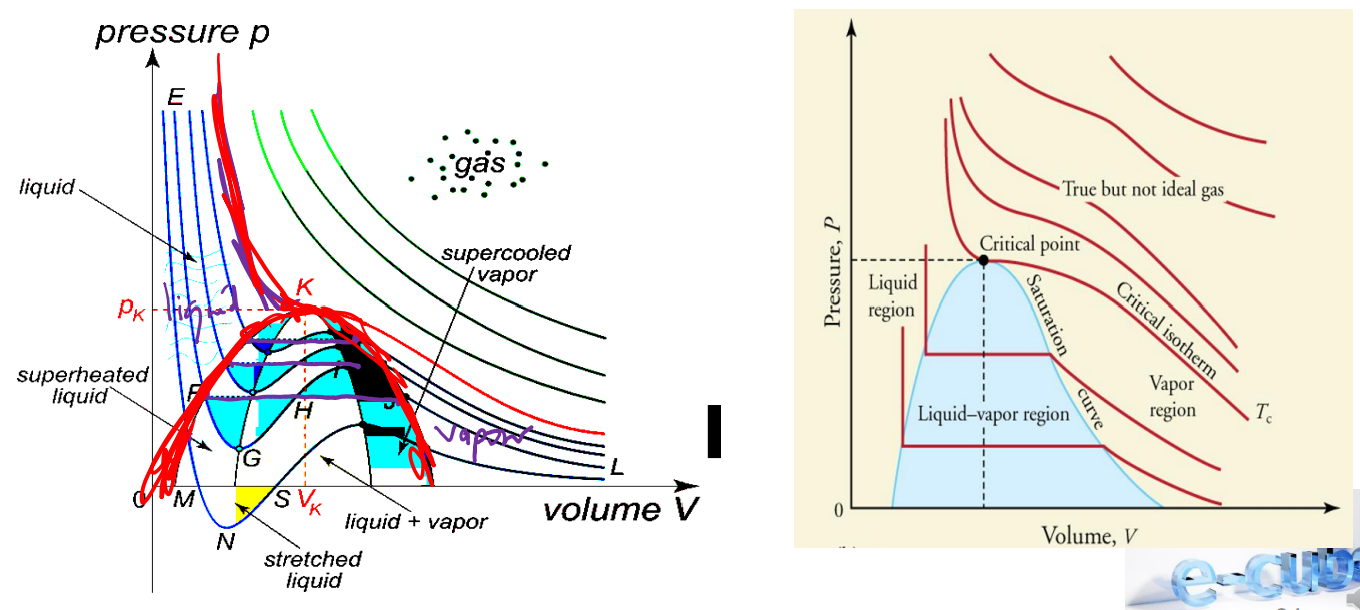
\includegraphics[width = 0.7\textwidth]{./img/figure18.png}
	\caption{Van der Waals.}
\end{figure}
\subsubsection{Link between molecular and microscopic}
Most of the important 19th century breakthroughs were determining link between macroscopic (could be seen) and microscopic (could not be seen). For example, Brownian motion:
\begin{gather}
	\frac{RT}{5\pi\mu dN_A} = D = \lim_{t\rightarrow \infty} \frac{\left(x^2\right)}{2t} \approx \SI{10e-10}{\meter\squared\per\second}
\end{gather}
This represented a link between Avogadro's constant and macroscopic movement of particles. Here $N_A = \SI{6e23}{\per\mole}$. Theory by Einstein (1905) and Sutherland (1905). Millikans experiments: determination of the charge on an electron. The link between molecular and microscopic last areas of modern science to be worked out.
\subsubsection{Einstein theory and Millikans experiment}
Based around kinetic theory of gases and momentum change due to collision. Pressure is a manifestation of a:
\begin{gather}
	P = \frac{2}{3}\frac{N}{V}\frac{1}{2}m_0 \overline{v}^2\\
	\therefore PV = nRT = \frac{N}{N_a}RT = Nk_BT\\
	\therefore KE = \frac{3}{2}Nk_bT = \frac{3}{2}nRT = \frac{NDF}{2}nRT
\end{gather}
where $NDF$ is number of degrees of freedom.
\subsubsection{Model assumptions}
\begin{itemize}
	\item No intermolecular forces between the gas particles
	\item The volume occupied by the particles is negligible compared to the volume of the container they occupy
	\item The only interactions between the particles and with the container walls are perfectly elastic collisions.
	\item Real gas, the atoms or molecules have a finite size, and at close range they interact with each other through a variety of intermolecular forces, including dipole-dipole interactions, dipole induced dipole interactions and van der Waal's (induced dipole - induced dipole) interactions
	\item When applied to real gases, the ideal gas model breaks down when molecular size effects or intermolecular forces become important. This occurs under conditions of high pressure , when the molecules are forced close together and therefore interact strongly, and at low temperatures, when the molecules are moving slowly and intermolecular forces have a long time to act during a collision
\end{itemize}
The pressure at which the ideal gas model starts to break down will depend on the nature and strength of the intermolecular forces between the gas particles, and therefore on their identity. The ideal gas model becomes more and more exact as the pressure is lowered, since at very low pressures the gas particles are widely spaced apart and interact very little with each other.
\begin{gather}
	\textrm{number density } = \frac{N}{V} = \frac{nN_A}{V}\\
	\Delta p_x = \left(2mv_x\right)\left(\frac{1}{2}\frac{nN_a}{V}Av_x \Delta t\right) = \frac{nMAv_x^2 \Delta t}{V}\\
	p = \frac{F_x}{A} = \frac{nMv_x^2}{V}
\end{gather}
\section{Chemistry for engineers}
Chemistry has a molecular origin. The engineering challenge is how to include chemistry into multi-physics problems. Chemistry might be simple:
\begin{gather}
	\ce{NaOH + HCl -> NaCl + H2O}
\end{gather}

%\newpage
%\bibliographystyle{unsrtnat}
%\bibliography{Refs.bib}
%\appendix
\chapter{Plots}
\begin{figure}[H]
    \centering
    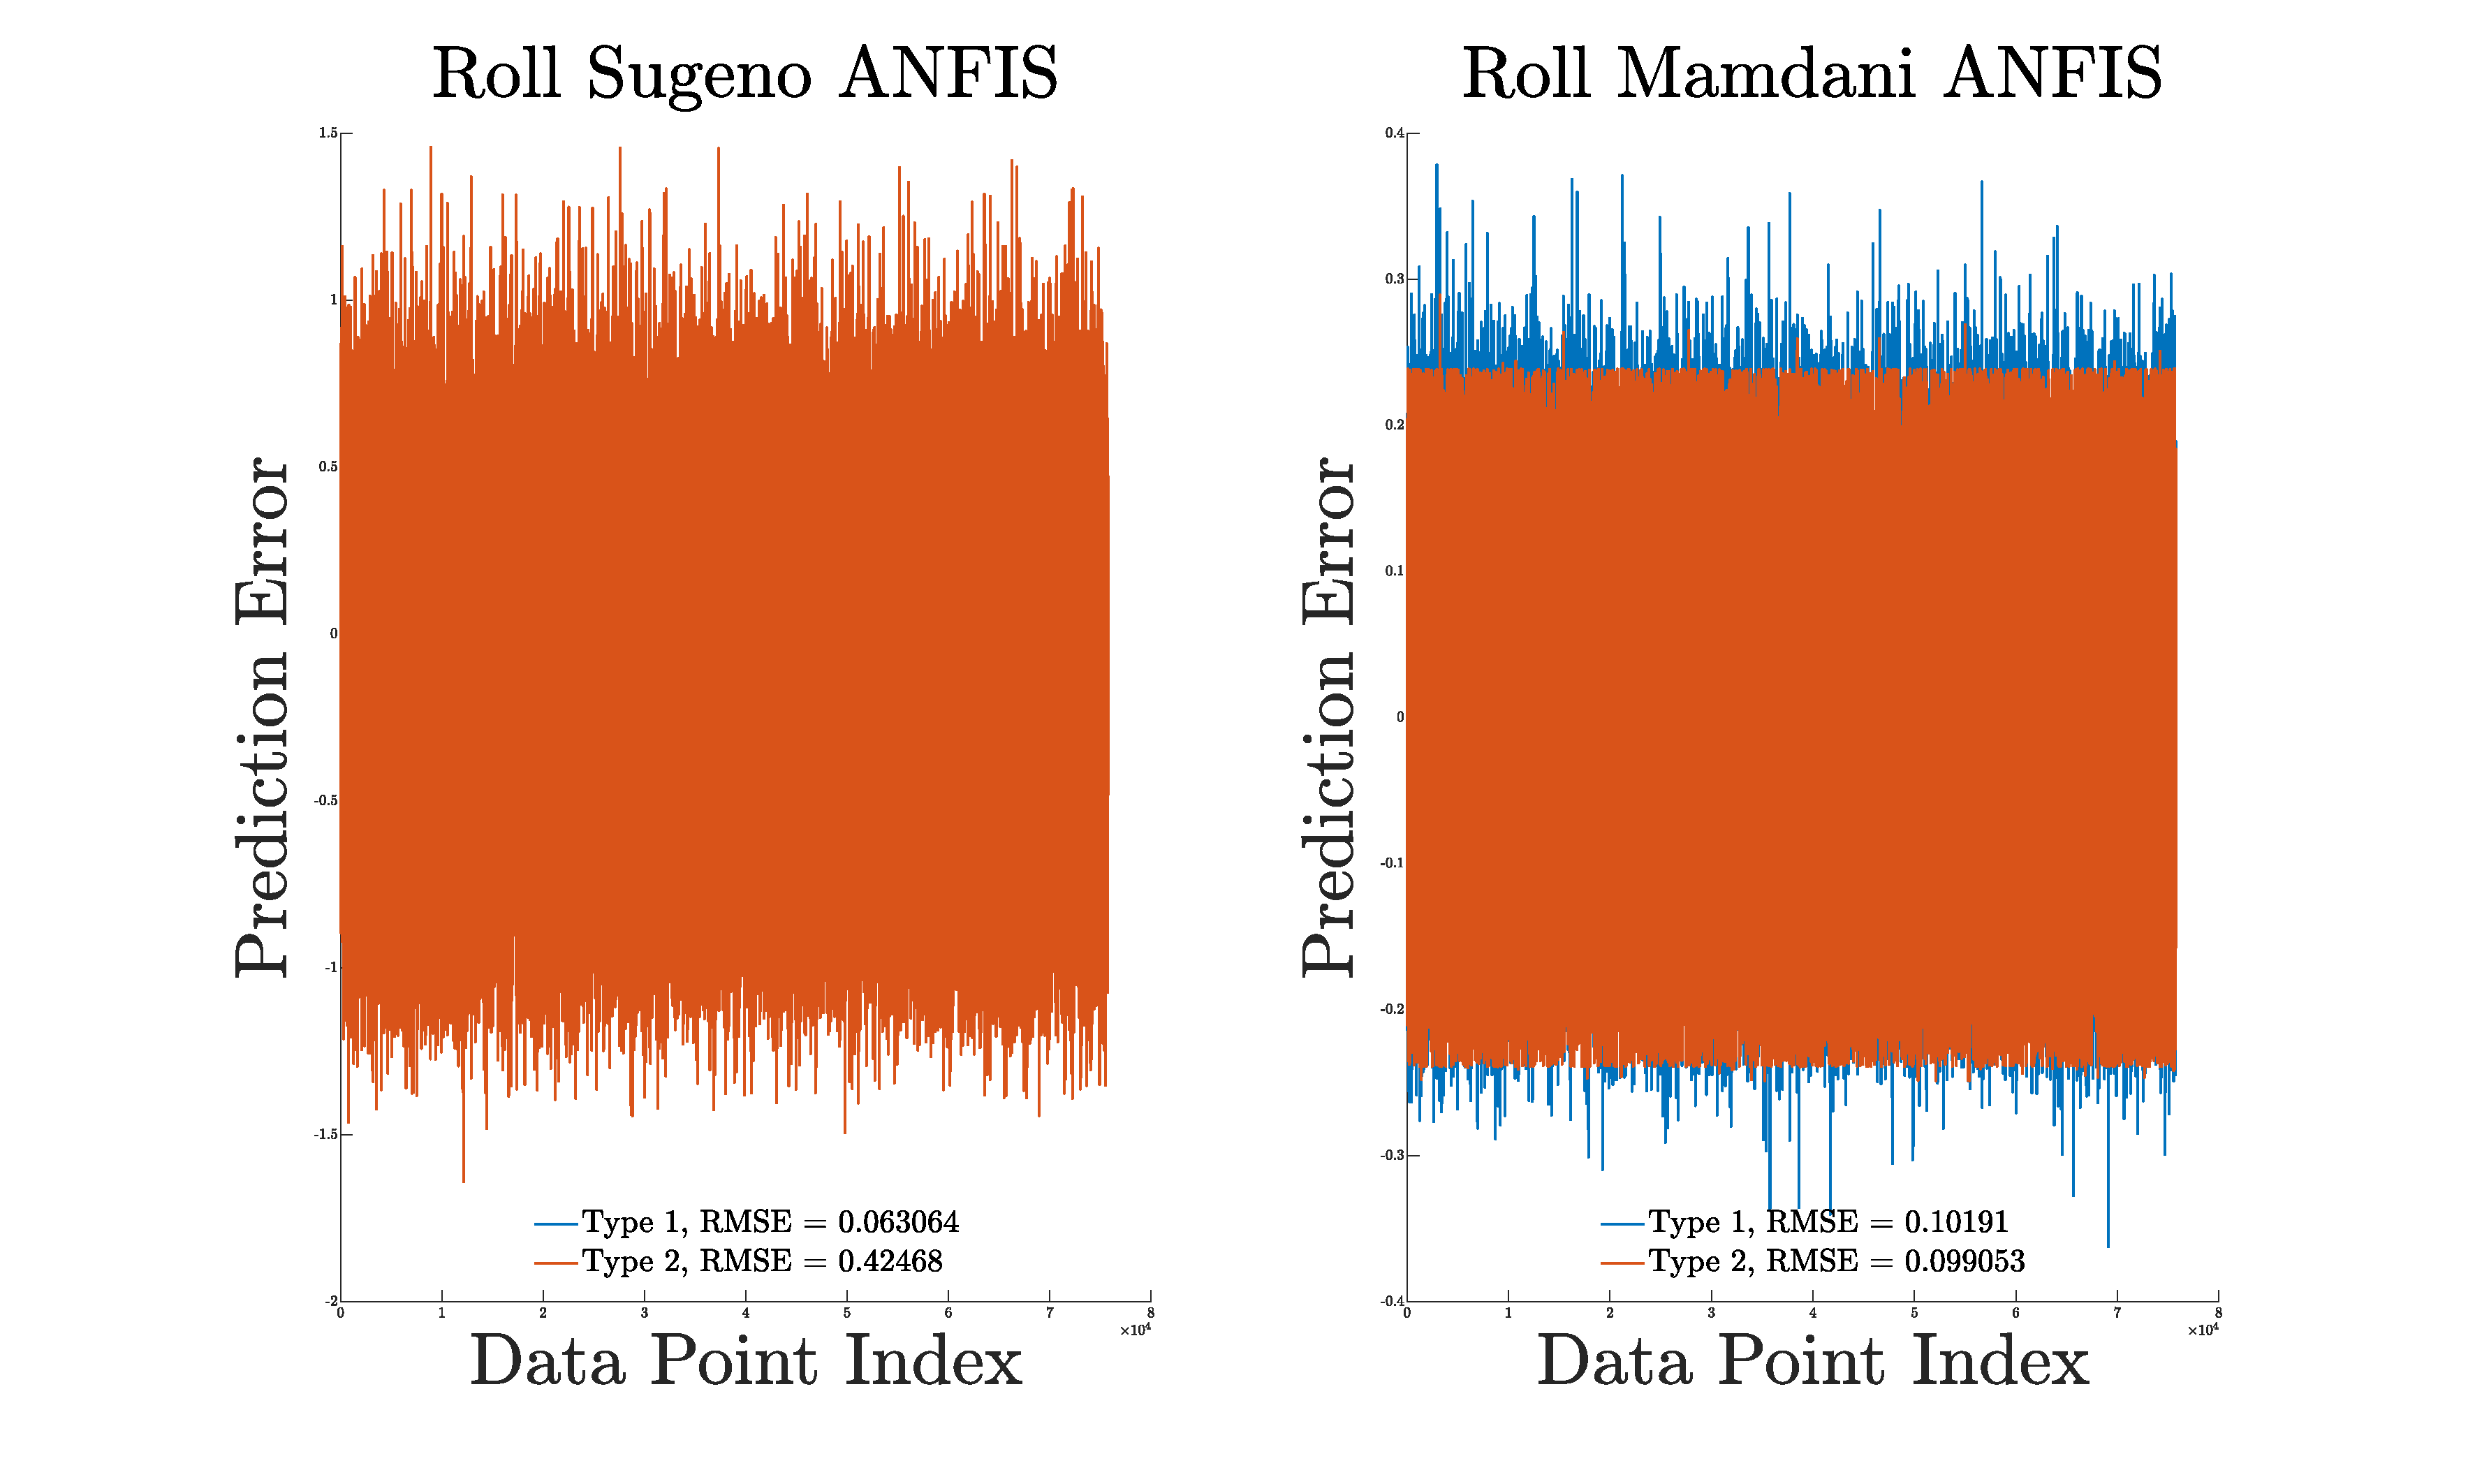
\includegraphics[width = 0.8\textwidth]{img/Roll Type.pdf}
    \caption{RMSE results for Type-1 and Type-2 Configurations for Roll Output}
    \label{fig:roll_type}
\end{figure}
\begin{figure}[H]
    \centering
    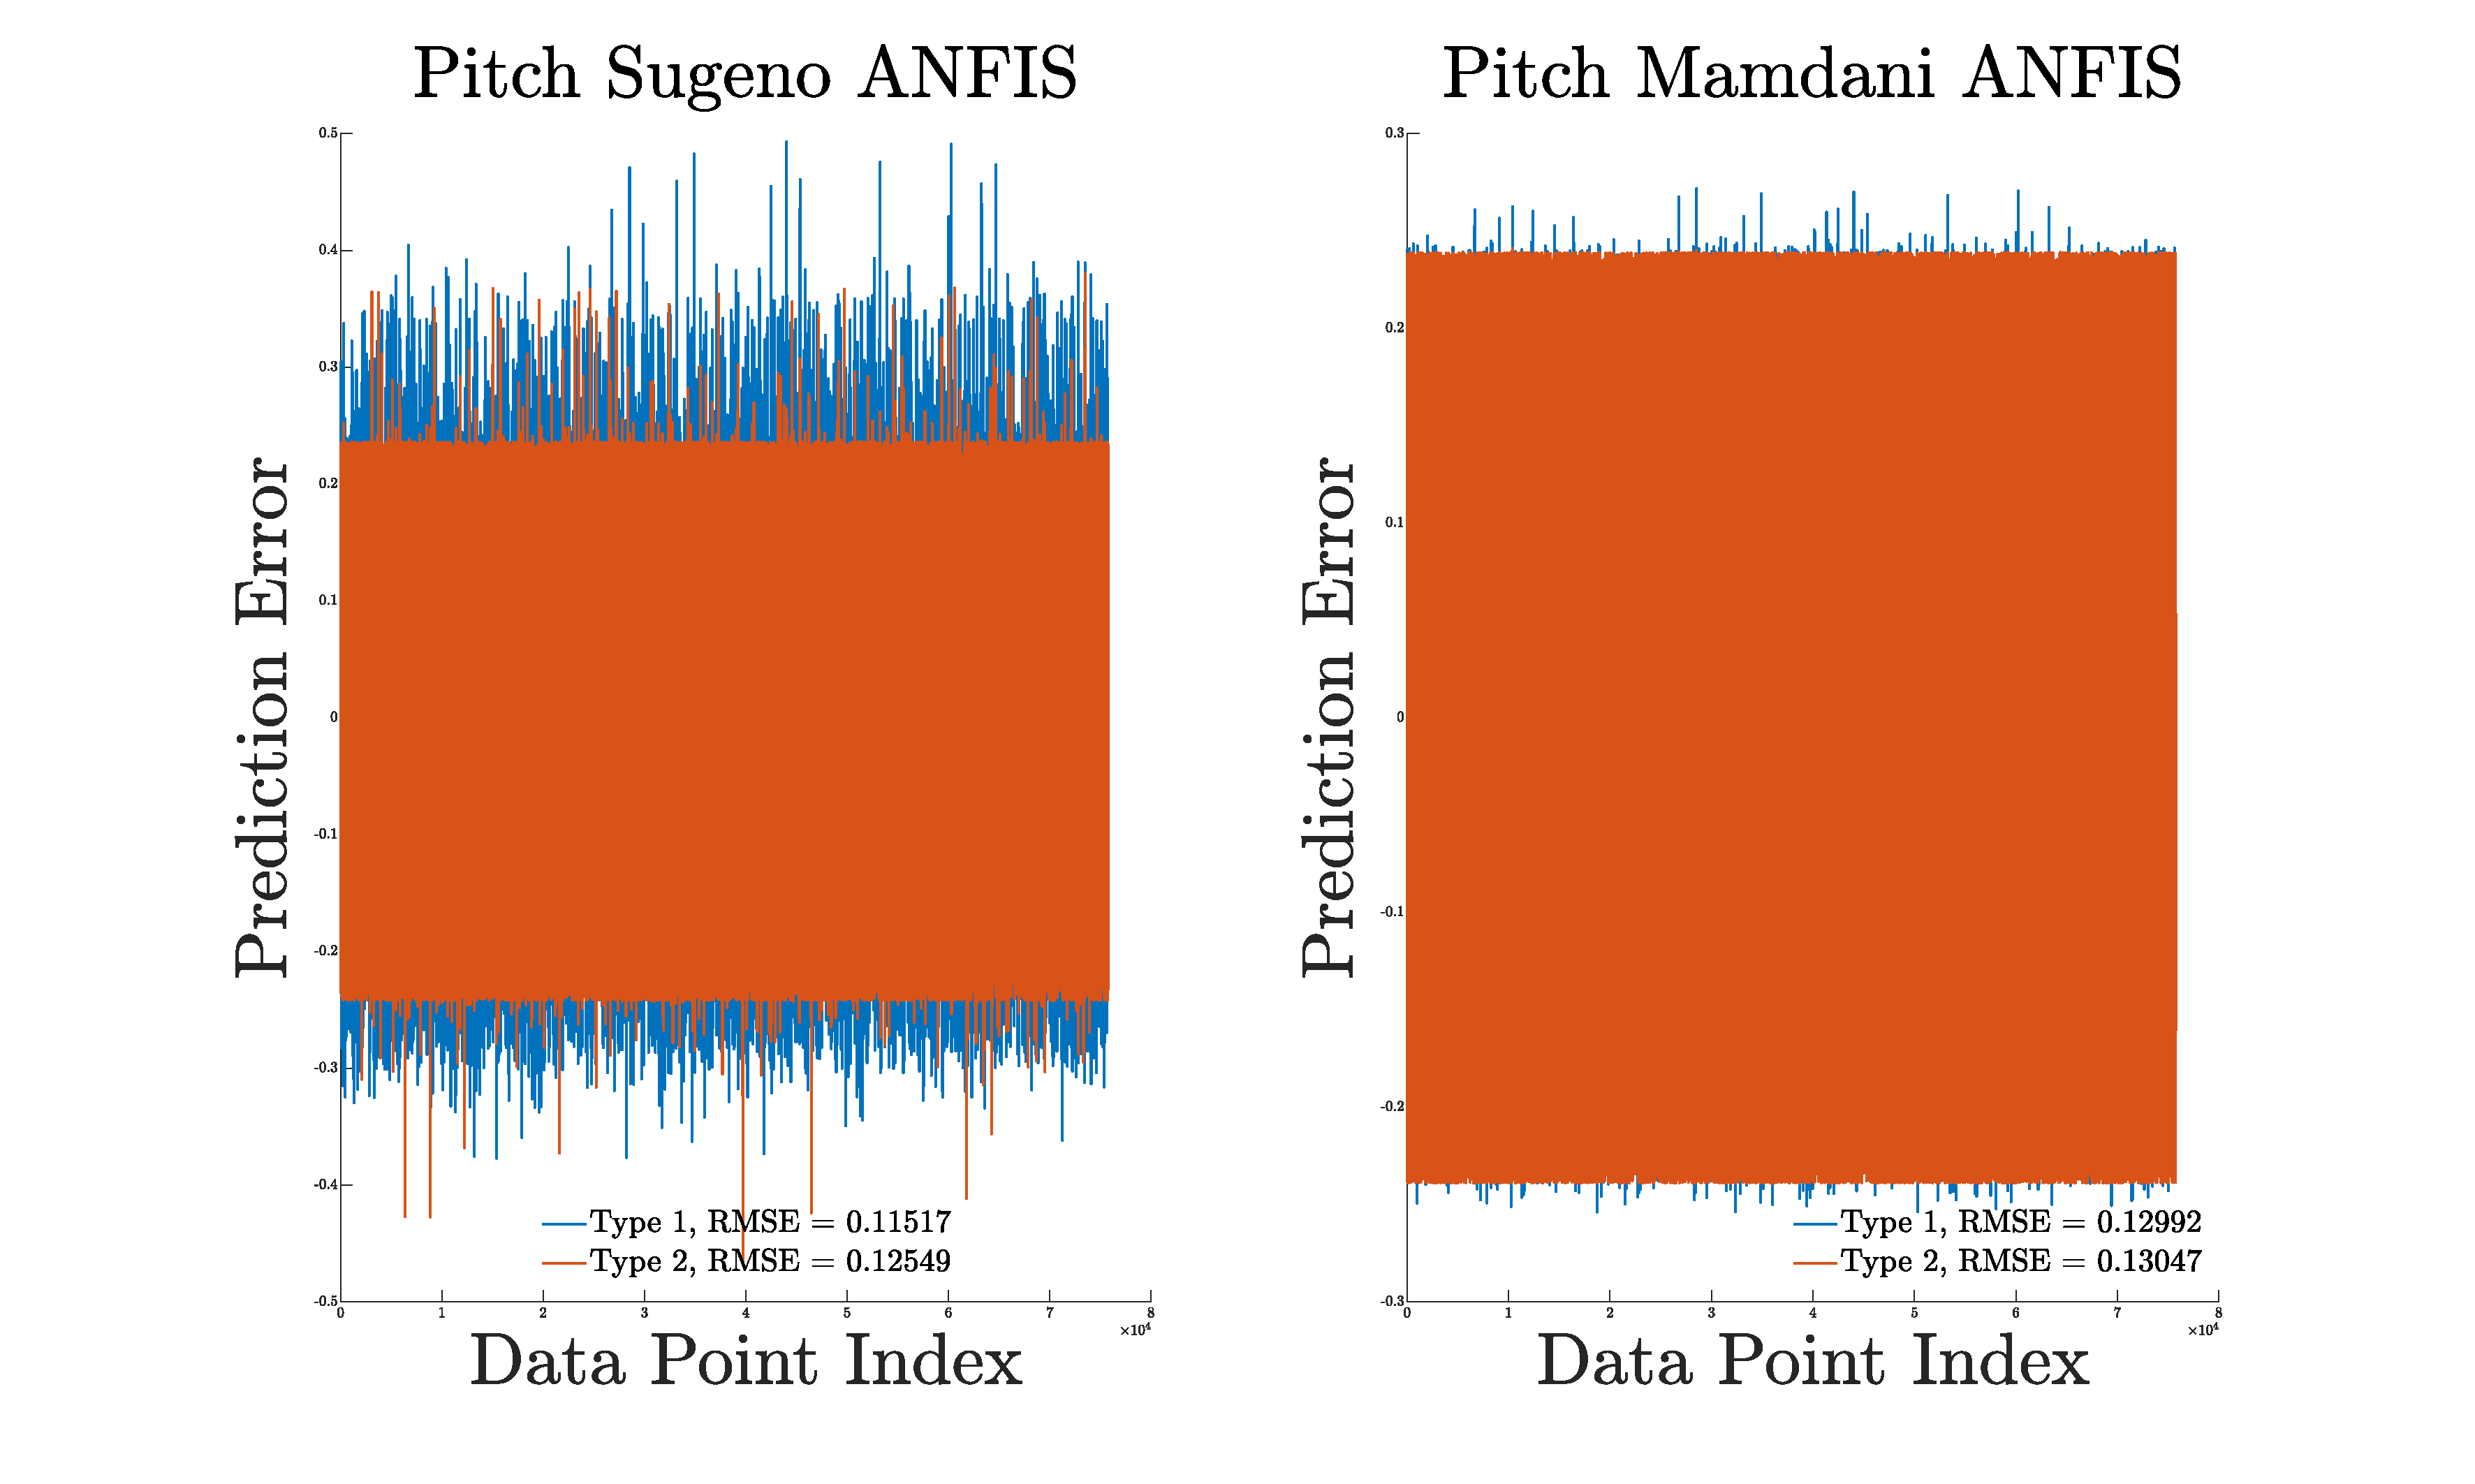
\includegraphics[width = 0.8\textwidth]{img/Pitch Type.pdf}
    \caption{RMSE results for Type-1 and Type-2 Configurations for Pitch Output}
    \label{fig:pitch_type}
\end{figure}
\begin{figure}[H]
    \centering
    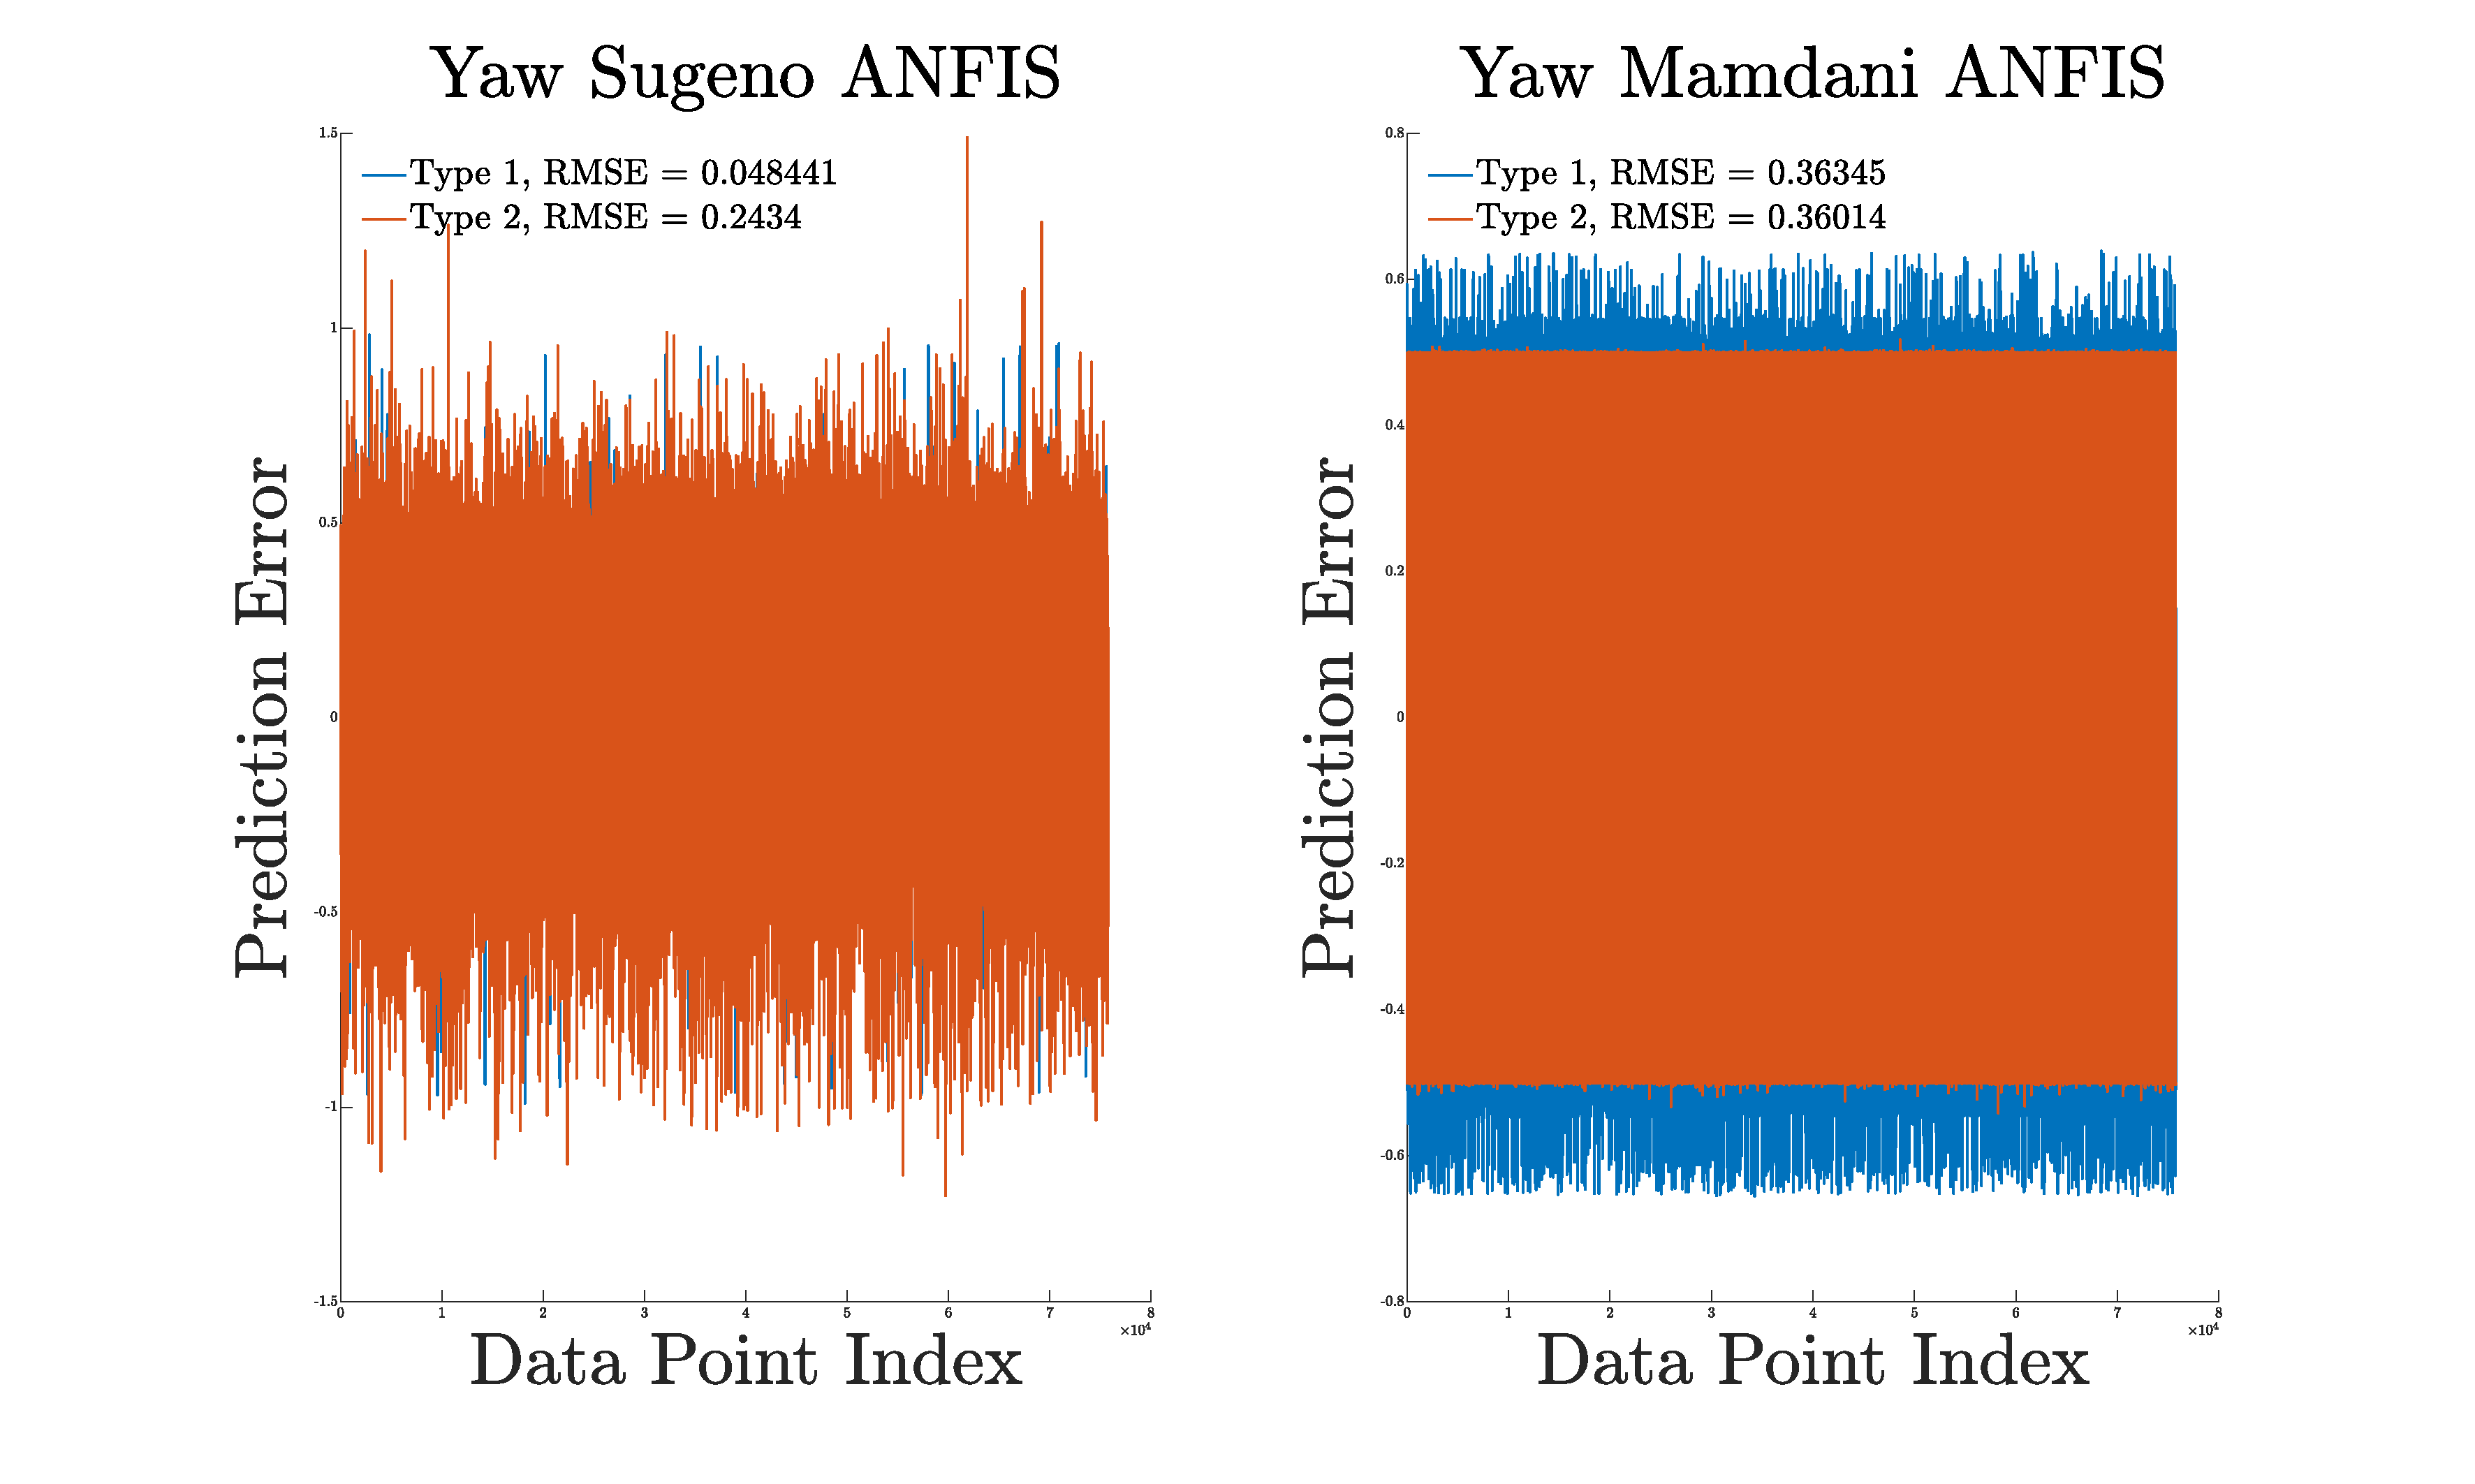
\includegraphics[width = 0.6\textwidth]{img/Yaw Type2.pdf}
    \caption{RMSE results for Type-1 and Type-2 Configurations for Yaw Output}
    \label{fig:yaw_type}
\end{figure}
\begin{figure}[H]
    \centering
    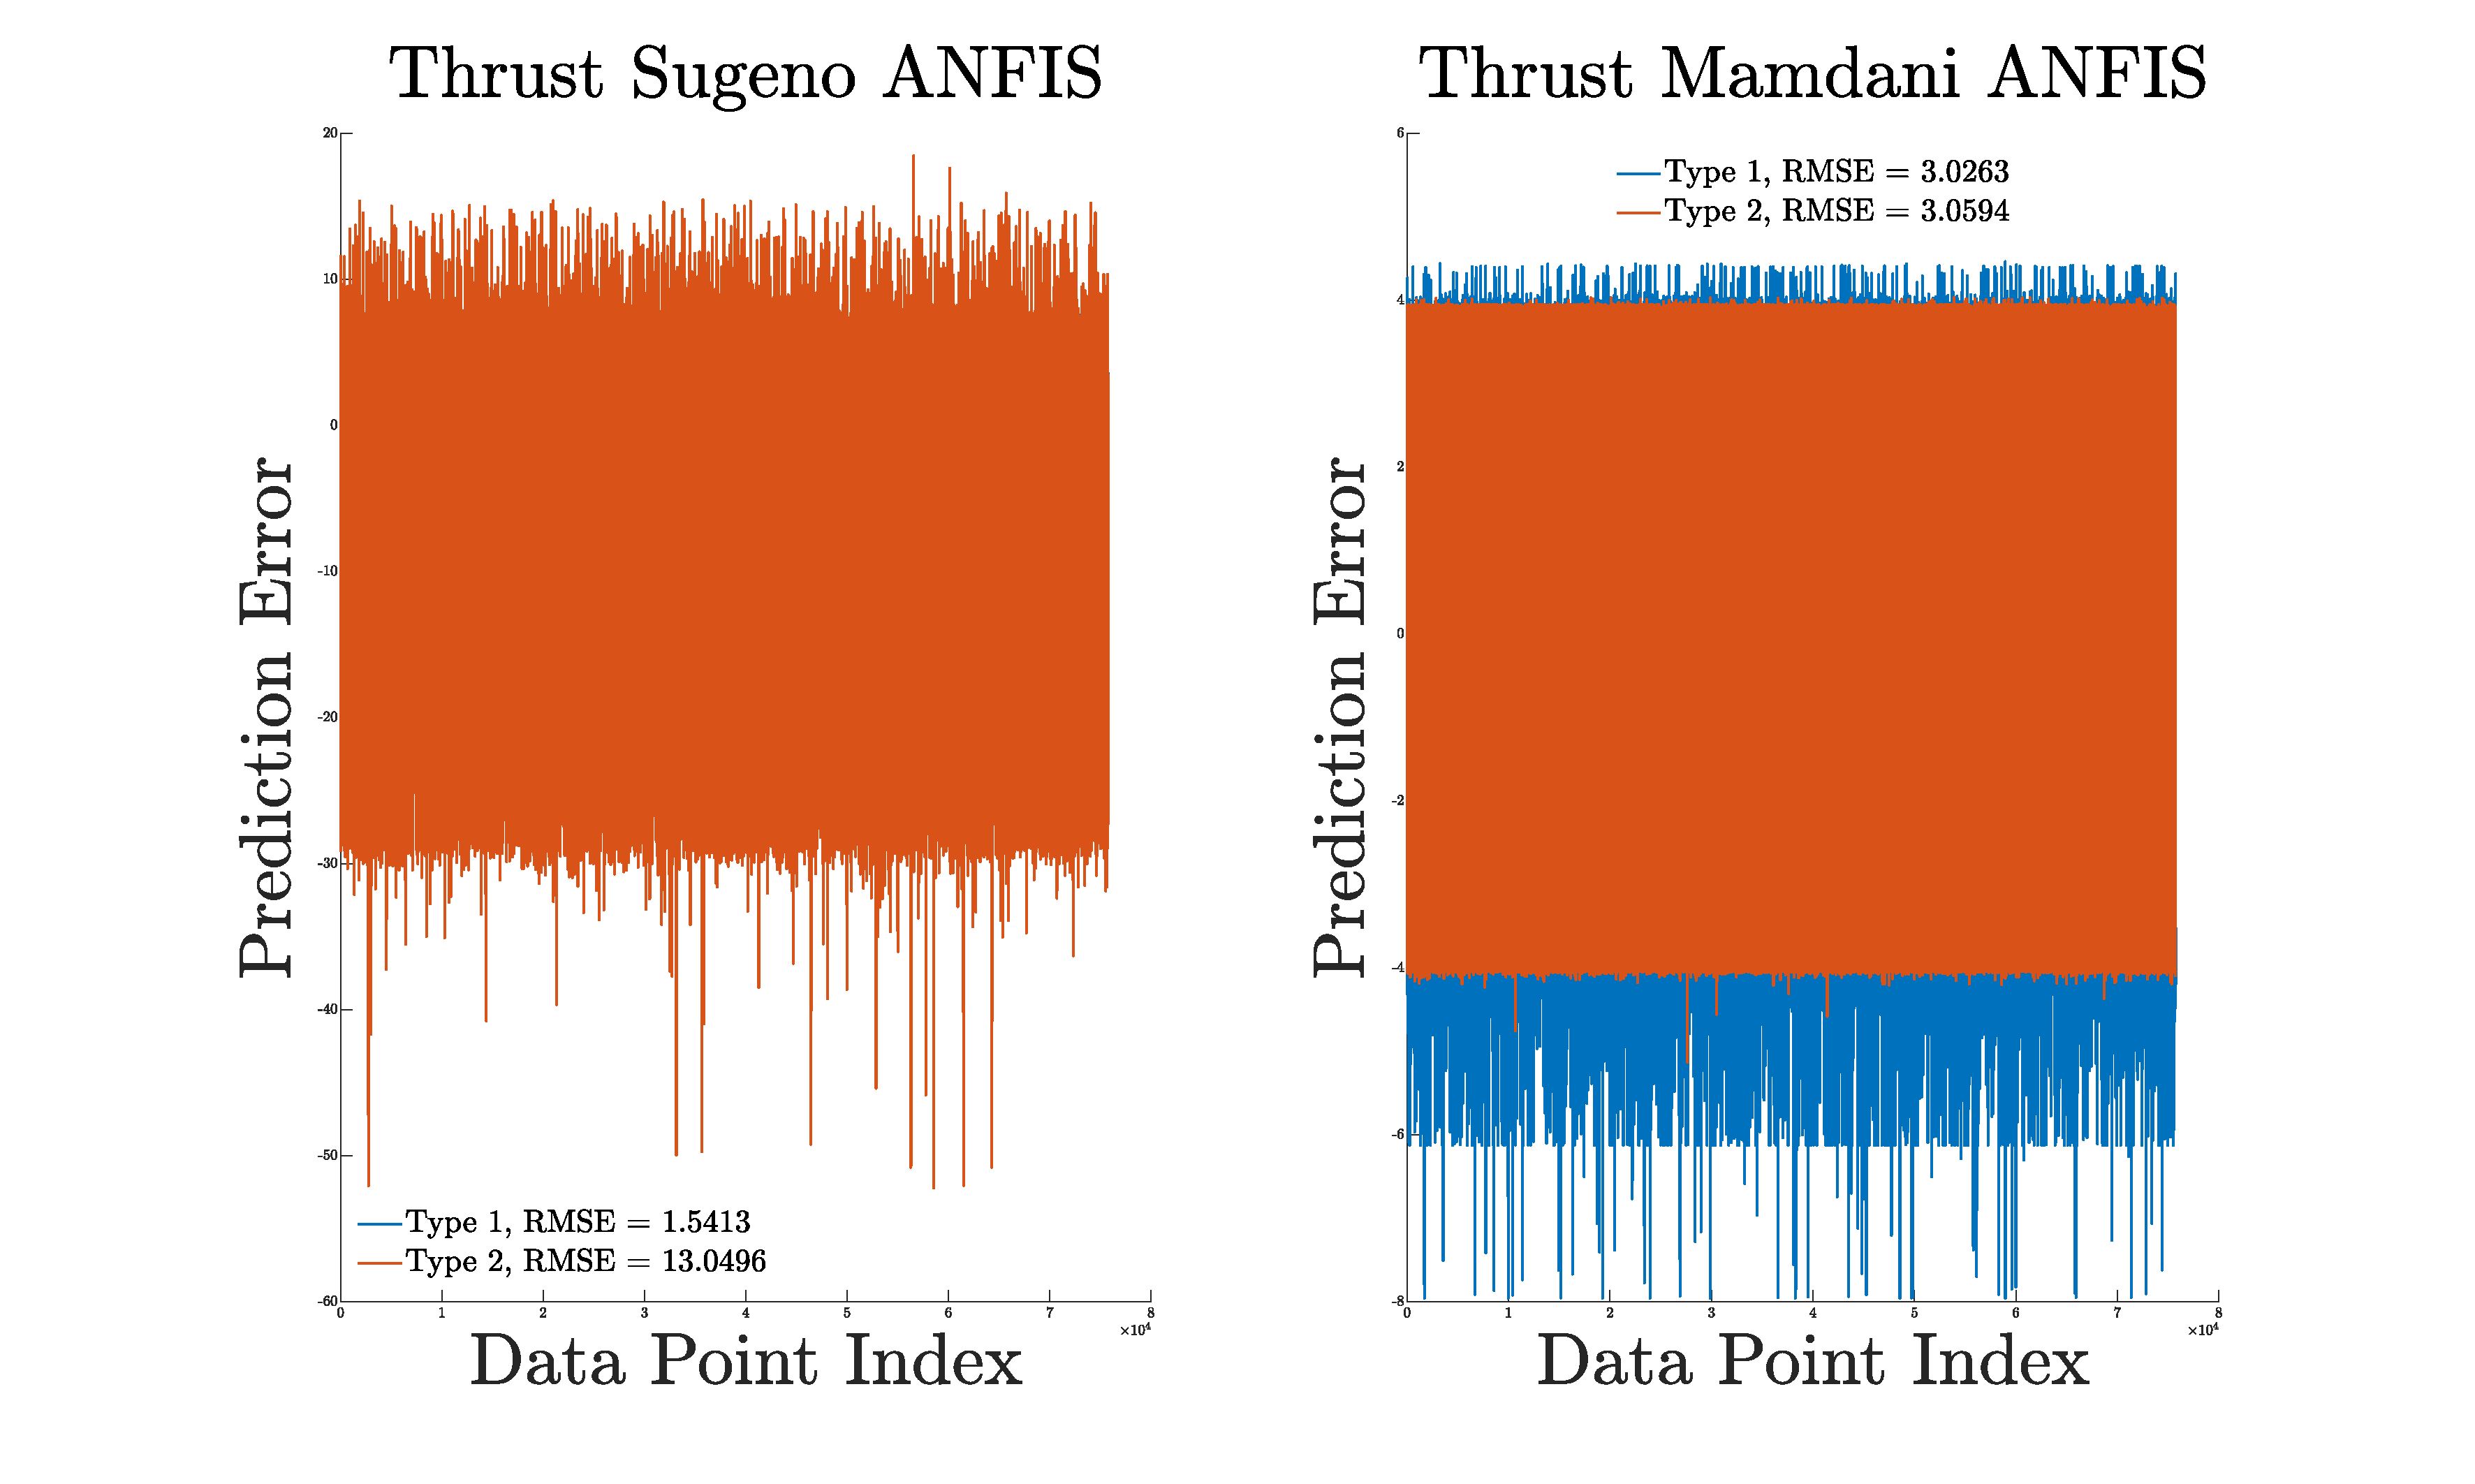
\includegraphics[width = 0.6\textwidth]{img/Thrust Type.pdf}
    \caption{RMSE results for Type-1 and Type-2 Configurations for Thrust Output}
    \label{fig:thrust_type}
\end{figure}
\begin{figure}[H]
    \centering
    \begin{minipage}[b]{0.45\textwidth}
        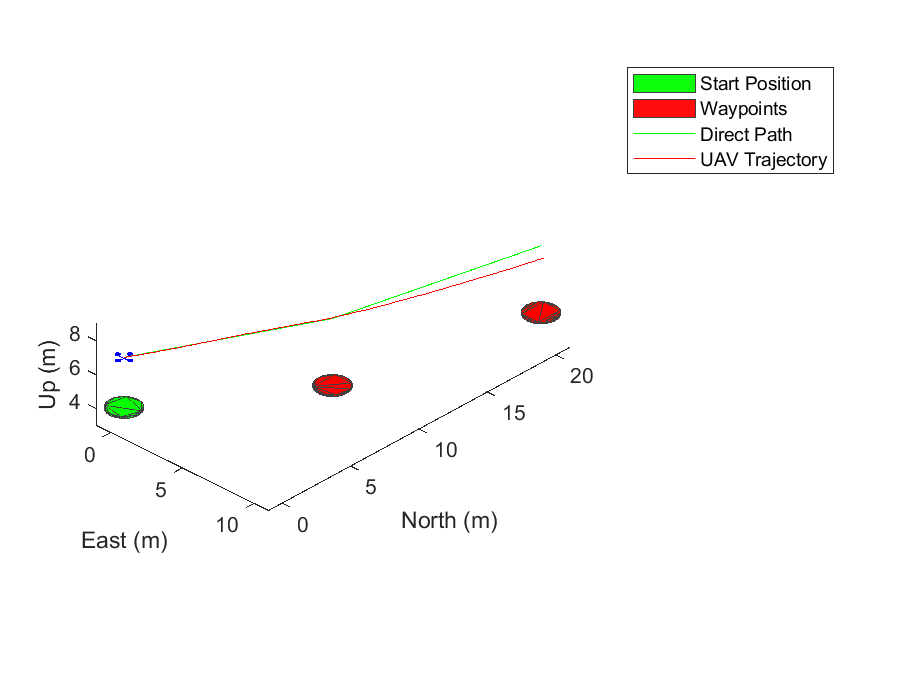
\includegraphics[height=5cm,keepaspectratio]{img/scenario1_pid_paths.eps}
        \caption{Scenario 1 Path taken using PID Drone Control}
        \label{fig:Paths1_pid}
    \end{minipage}
    \hfill
    \begin{minipage}[b]{0.45\textwidth}
        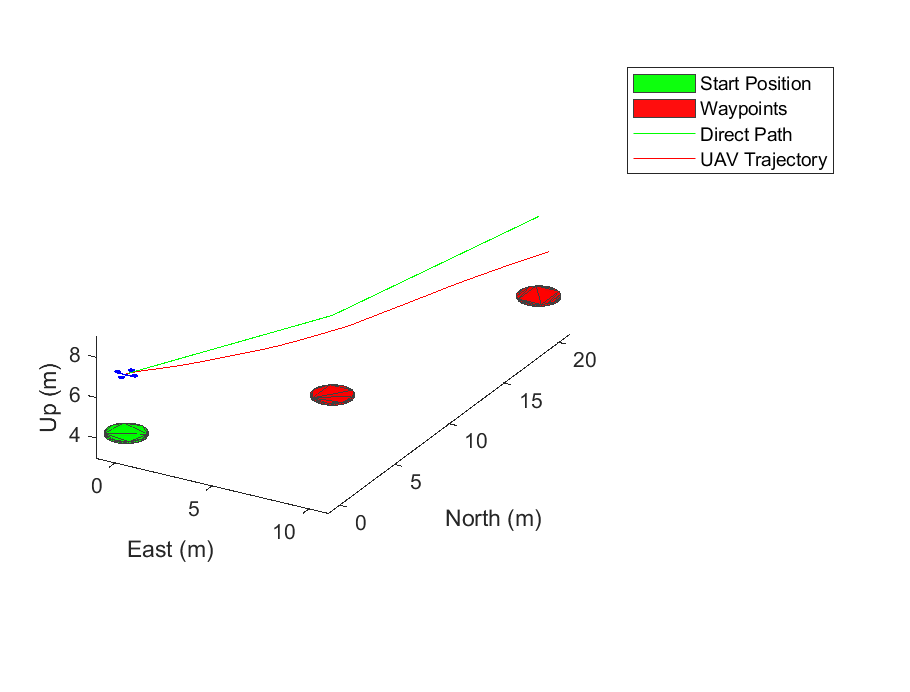
\includegraphics[height=5cm,keepaspectratio]{img/scenario1_fis_paths.eps}
        \caption{Scenario 1 Path taken using ANFIS Drone Control}
        \label{fig:Paths1_fis}
    \end{minipage}
\end{figure}
\begin{figure}[H]
    \centering
    \begin{minipage}[b]{0.45\textwidth}
        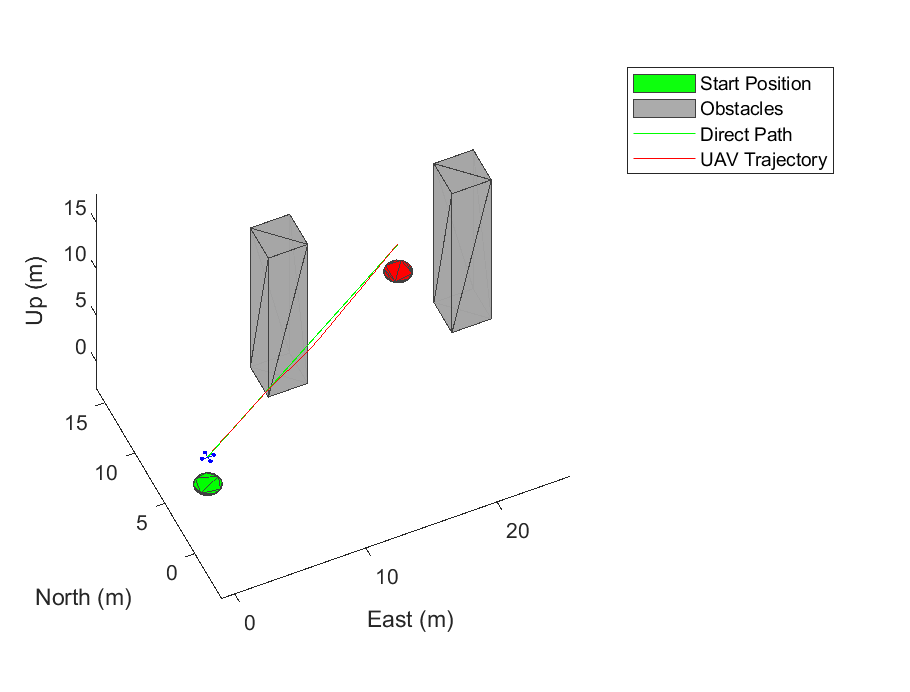
\includegraphics[height=5cm,keepaspectratio]{img/scenario2_pid_paths.eps}
        \caption{Scenario 2 Path taken using PID Drone Control}
        \label{fig:Paths2_pid}
    \end{minipage}
    \hfill
    \begin{minipage}[b]{0.45\textwidth}
        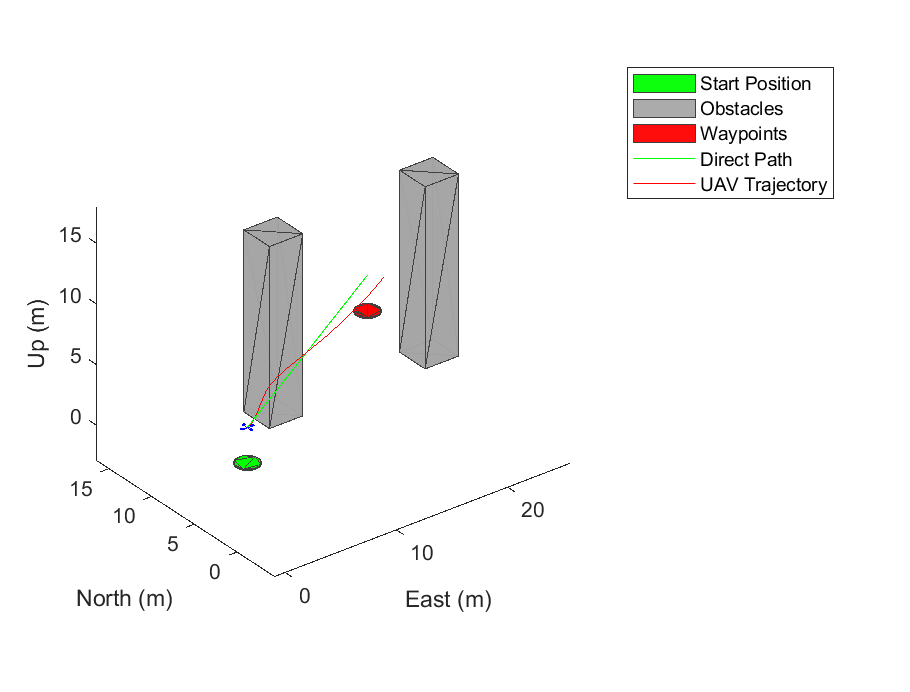
\includegraphics[height=5cm,keepaspectratio]{img/scenario2_fis_paths.eps}
        \caption{Scenario 2 Path taken using ANFIS Drone Control}
        \label{fig:Paths2_fis}
    \end{minipage}
\end{figure}
\begin{figure}[H]
    \centering
    \begin{minipage}[b]{0.45\textwidth}
        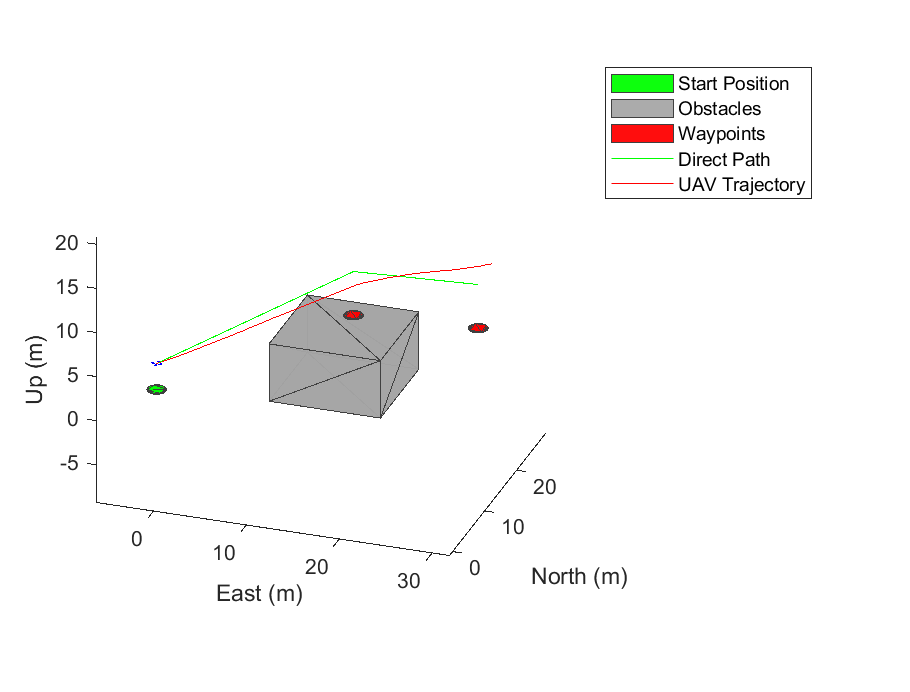
\includegraphics[height=5cm,keepaspectratio]{img/scenario3_pid_paths.eps}
        \caption{Scenario 3 Path taken using PID Drone Control}
        \label{fig:Paths3_pid}
    \end{minipage}
    \hfill
    \begin{minipage}[b]{0.45\textwidth}
        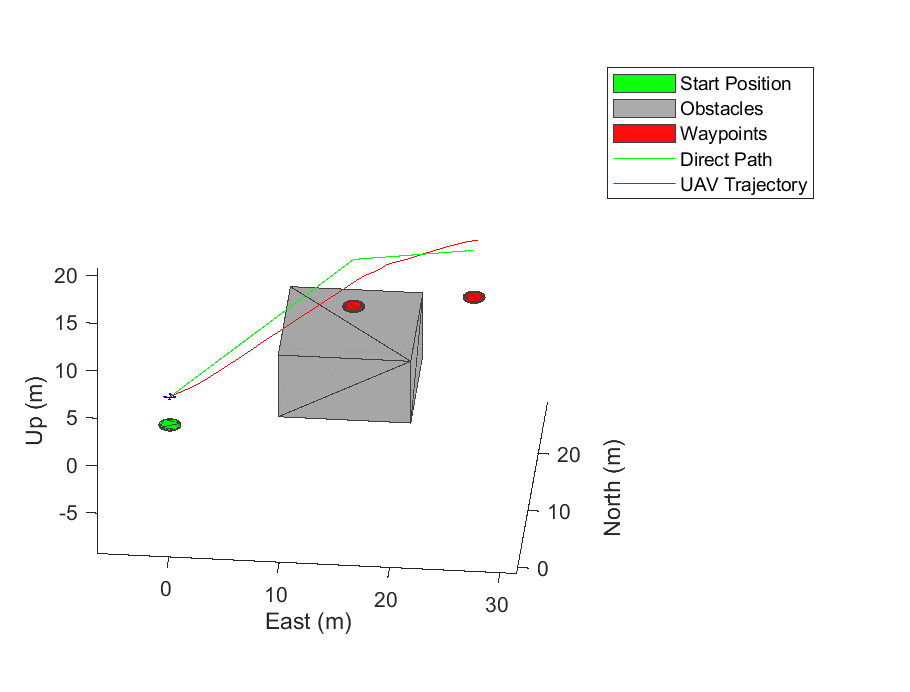
\includegraphics[height=5cm,keepaspectratio]{img/scenario3_fis_paths.eps}
        \caption{Scenario 3 Path taken using ANFIS Drone Control}
        \label{fig:Paths3_fis}
    \end{minipage}
\end{figure}
\begin{figure}[H]
    \centering
    \begin{minipage}[b]{0.45\textwidth}
        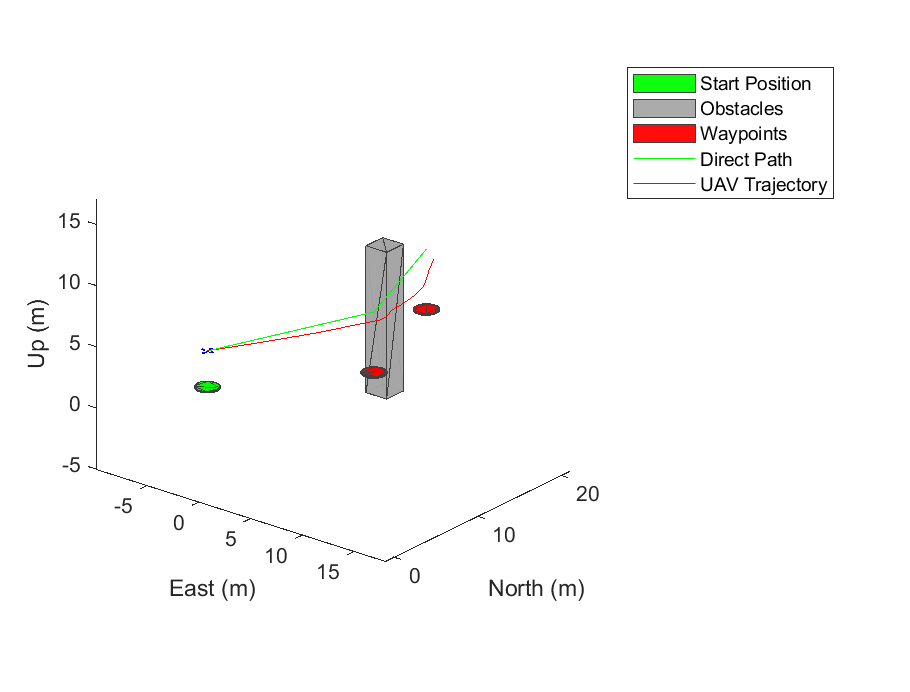
\includegraphics[height=5cm,keepaspectratio]{img/scenario4_pid_paths.eps}
        \caption{Scenario 4 Path taken using PID Drone Control}
        \label{fig:Paths4_pid}
    \end{minipage}
    \hfill
    \begin{minipage}[b]{0.45\textwidth}
        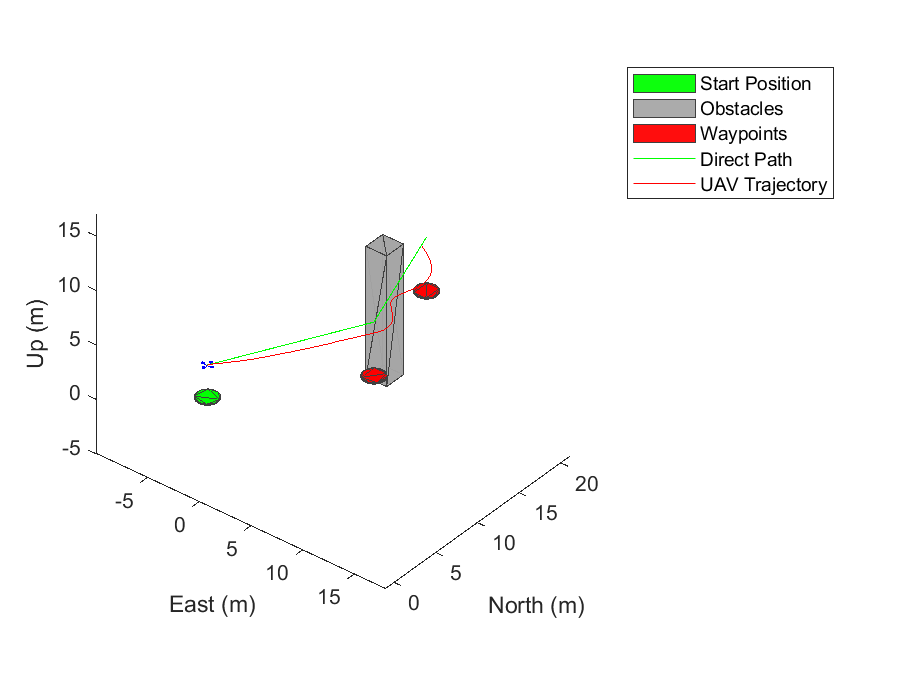
\includegraphics[height=5cm,keepaspectratio]{img/scenario4_fis_paths.eps}
        \caption{Scenario 4 Path taken using ANFIS Drone Control}
        \label{fig:Paths4_fis}
    \end{minipage}
\end{figure}
\begin{figure}[H]
    \centering
    \begin{minipage}[b]{0.45\textwidth}
        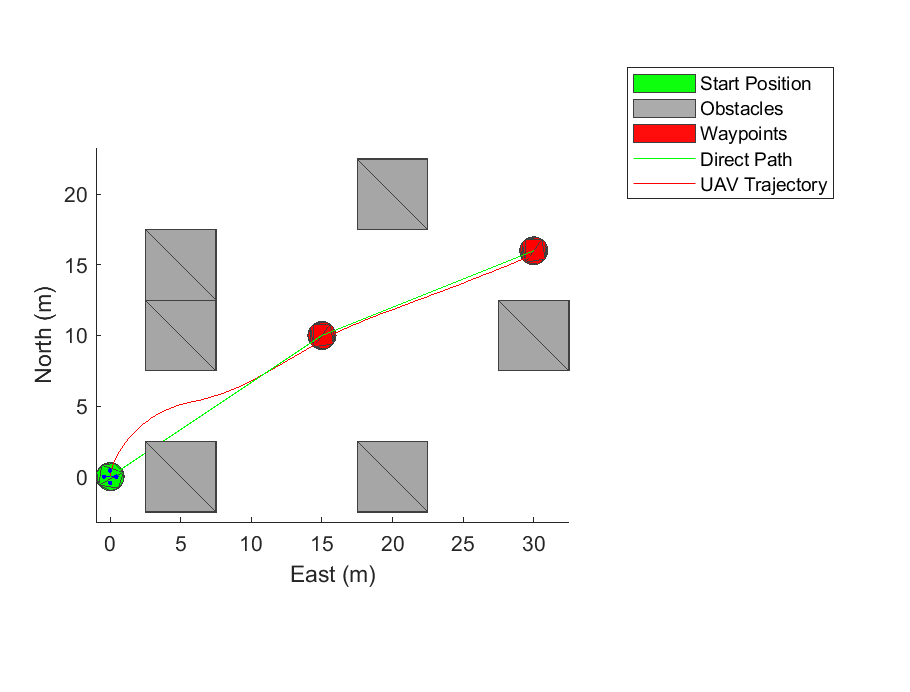
\includegraphics[height=5cm,keepaspectratio]{img/scenario5_pid_paths.eps}
        \caption{Scenario 5 Path taken using PID Drone Control}
        \label{fig:Paths5_pid}
    \end{minipage}
    \hfill
    \begin{minipage}[b]{0.45\textwidth}
        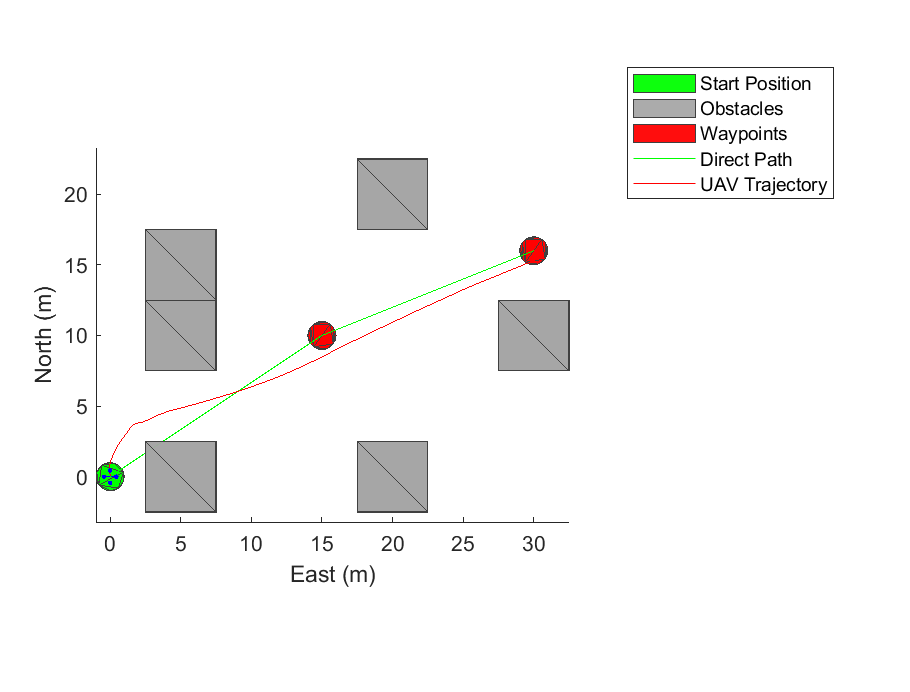
\includegraphics[height=5cm,keepaspectratio]{img/scenario5_fis_paths.eps}
        \caption{Scenario 5 Path taken using ANFIS Drone Control}
        \label{fig:Paths5_fis}
    \end{minipage}
\end{figure}

\end{document}